\documentclass[10pt]{scrreprt}
\usepackage[utf8]{inputenc}
\usepackage{amsfonts}
\usepackage{amsmath}
\usepackage{amssymb}
\usepackage{commath}
\usepackage[ngerman]{babel}
\usepackage{enumitem}
\usepackage{booktabs}
\usepackage{longtable}
\usepackage{relsize}
\usepackage{pgfplots}
\usepackage{csvsimple}
\usepackage{pgfplotstable}
\usepackage{siunitx}
\usepackage{fancyhdr}
\usepackage{color}
\usepackage{float}
\usepackage{listings}

\definecolor{mygreen}{RGB}{28,172,0} % color values Red, Green, Blue
\definecolor{mylilas}{RGB}{170,55,241}


\lstset{language=Matlab,%
    %basicstyle=\color{red},
    breaklines=true,%
    morekeywords={matlab2tikz},
    keywordstyle=\color{blue},%
    morekeywords=[2]{1}, keywordstyle=[2]{\color{black}},
    identifierstyle=\color{black},%
    stringstyle=\color{mylilas},
    commentstyle=\color{mygreen},%
    showstringspaces=false,%without this there will be a symbol in the places where there is a space
    %numbers=left,%
    %numberstyle={\tiny \color{black}},% size of the numbers
    %numbersep=9pt, % this defines how far the numbers are from the text
    emph=[1]{for,end,break},emphstyle=[1]\color{red}, %some words to emphasise
    %emph=[2]{word1,word2}, emphstyle=[2]{style},
}

\setlength\parindent{0pt}

\setcounter{chapter}{2}
\setcounter{secnumdepth}{3}


\pagestyle{fancy}
\fancyhf{}
\lhead{GPET Versuch 3}
\rhead{Tim Luchterhand, Paul Nykiel}
\cfoot{\thepage}

\author{Tim Luchterhand, Paul Nykiel \protect\\ tim.luchterhand@uni-ulm.de, paul.nykiel@uni-ulm.de}
\title{GPET Versuch 3 --- Transformieren und Telefonieren mit Fourier}
\subtitle{Gruppe: Dienstag14}

\begin{document}
        \maketitle
        \chapter{Vorbereitende Aufgaben}
        \section{Signaleigenschaften und Signalklassifikation}
        \subsection{Signalklassifikation}
        \paragraph{Aufgabe}
        Um welche Art von Signaltypen handelt es sich bei den Signalen in Abbildung 11?

        \paragraph{Lösung}
        \begin{itemize}
            \item $a(t)$: harmonisch, periodisch, deterministisch
            \item $b(t)$: deterministisch
            \item $c(t)$: stochastisch
            \item $d(t)$: periodisch, deterministisch
        \end{itemize}

        \subsection{Harmonische Signale}
        \paragraph{Aufgabe}
        Bestimmen Sie die Frequenz $f$, Periode $T$ und Nullphasenverschiebung $\phi_0$ des harmonischen
        Signals $x_4(t)$ aus Abbildung 4. Wie auf Seite 6 beschrieben, handelt es sich hierbei
        um eine verschoben cos-Funktion. Zeichnen Sie die Frequenz in Diagramm ähnlich wie
        Abbildung 12 ein.

        \paragraph{Lösung}
        \begin{eqnarray*}
            f &=& 1\si{\hertz}\\
            T &=& 1\si{\second}\\
            \phi_0 &=& -\frac{\pi}{2}
        \end{eqnarray*}

        \begin{center}
            \begin{figure}[H]
                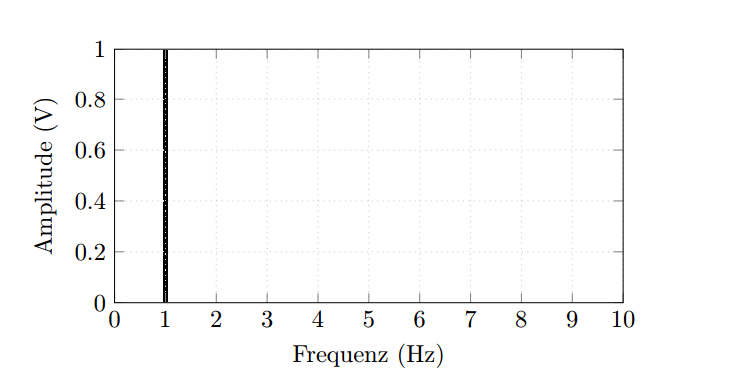
\includegraphics[width=\textwidth]{vorbereitenderBullshit.png}
              %\caption{Oszilloskop Screenshot}
            \end{figure}
        \end{center}

        \subsection{Elektrische Signal}
        \paragraph{Aufgabe}
        Bestimmen Sie die Amplitude $\hat{x}$, den Effektivwert $x_{eff}$, den Spitze-Spitze Wert $x_{ss}$ und
        den Offset $\bar{x}$ des elektrischen Signals $x_5(t)$ aus Abbildung 5.

        \paragraph{Lösung}
        \begin{eqnarray*}
            \hat{x} &=& 1\si{\volt}\\
            x_{eff} &=& 0.7\si{\volt}\\
            x_{ss} &=& 2\si{\volt}\\
            \bar{x} &=& 0.3\si{\volt}\\
        \end{eqnarray*}


        \section{Transformation in den Frequenzbereich}
        \subsection{Bandbreite}
        \paragraph{Aufgabe}
        Bestimmen Sie die obere und untere Grenzfrequenz $f_2$ und $f_1$ und daraus die Bandbreite
        der Signale aus Abbildung 13. Dabei sollen die Definitionen der 3dB Grenzfrequenzen
        gelten. Hinweis: Bei den Signalen handelt es sich um von Musikinstrumenten gespielte
        Töne.

        \paragraph{Lösung}
        \subparagraph{$A(f)$}
        \begin{eqnarray*}
            f_1 &=& 1050 \si{\hertz}\\
            f_2 &=& 2100 \si{\hertz}\\
            \Rightarrow B &=& 1050\si{\hertz}
        \end{eqnarray*}

        \subparagraph{$B(f)$}
        \begin{eqnarray*}
            f_1 &=& 1050 \si{\hertz}\\
            f_2 &=& 1500 \si{\hertz}\\
            \Rightarrow B &=& 450\si{\hertz}
        \end{eqnarray*}

        \subsection{Darstellung im Frequenzbereich}
        \paragraph{Aufgabe}
        Zeichnen Sie das Spektrum eines Signals mit den Frequenzen $f_1=3\si{\hertz}$ und $f_2=9\si{\hertz}$
        und den Amplituden $A_1 = 1\si{\volt}$ und $A_2 = 0.5\si{\volt}$ in ein Diagramm ein. Nutzen Sie dafür
        ein ähnliches Diagramm wie in Abbildung 12. Wie lautet die Signaldarstellung im Zeitbereich?

        \paragraph{Lösung}
        \begin{center}
            \begin{figure}[H]
                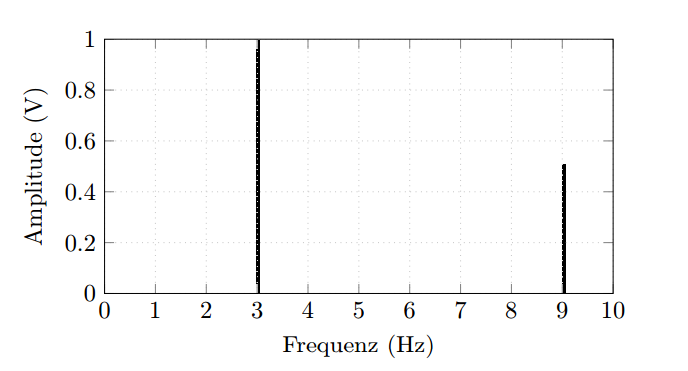
\includegraphics[width=\textwidth]{vorbereitenderBulldshit2.png}
              %\caption{Oszilloskop Screenshot}
            \end{figure}
        \end{center}

        \section{MATLAB}
        \paragraph{Aufgabe}
        Verschaffen Sie sich einen Überblick über die folgenden Kapitel im auf der Praktikumsseite
        bereitgestellten MATLAB Primer. Da im Praktikum mit MATLAB gearbeitet wird ist
        ein prinzipielles Verständnis von Oberfläche, Syntax und den angegebenen Funktionen
        elementar.

        \begin{itemize}
            \item \textbf{Beschreibung der Benutzeroberfläche:}

                Welche Bereiche gibt es? Wozu werden sie benutzt?
                \begin{itemize}
                    \item Konsole
                    \item Dateibaum
                    \item Letzte Befehle
                    \item Variablen
                \end{itemize}
            \item \textbf{Erste Schritte}

                Wie kann der Wert einer Variablen \glqq{}temp\grqq{} abgefragt werden?

                \texttt{>> temp}
            \item \textbf{Benutzung der MATLAB Hilfe}

                Wie lautet der Befehl um mehr Information (in HTML-Form) zur in MATLAB
                implemetierten FFT zu erhalten?

                \texttt{>> doc fft}

            \item \textbf{Zahlen, Vektoren, Matrizen}

                Wie kann auf die erste Zeile einer Matrix zugegriffen werden?

                \texttt{>> A(1,:)}

            \item \textbf{M-Files (Skripte/Funktionen)}

                Im Primer ist eine Funktion \texttt{fsummdiff(a,b)} gegeben. Wie erfolgt der Funktionsaufruf?
                Wie können beide Ausgabewerte in Variablen gespeichert werden?

                \texttt{>> [sum, diff] = fsummdiff(a, b)}

        \end{itemize}

        \subsection{FFT Auflösung}
        \paragraph{Aufgbae}
        Das im Praktikum verwendete Oszilloskop berechnet jeweils die FFT über das auf dem
        Schirm dargestellte Zeitsignal. Wie viele Perioden mussen dargestellt werden um die
        Frequenzauflösung zu vervierfachen, wenn auf dem Schirm 2 Perioden dargestellt werden?
        Wie lange ist anschließend die Dauer des Messintervalls, wenn die Signalfrequenz 1500 Hz
        beträgt? Wie groß ist die resultierende Frequenzauflösung?

        \paragraph{Lösung}
        Um die Frequenzauflösung zu vervierfachen, müssen 8 Perioden dargestellt werden.

        \begin{eqnarray*}
            N &=& 8\\
            f &=& 1500\si{\hertz}\\
            \Rightarrow T_{mess} &=& \frac{1}{f} \cdot N =  0.0053\si{\second}\\
            \Rightarrow f_{aufloesung} &=& \frac{1}{T_{mess}} = 187.5 \si{\hertz}
        \end{eqnarray*}

        \section{Mehrfrequenzwahlverfahren}
        \subsection{MFV-Signale im Zeitbereich}
        \paragraph{Aufgabe}
        Geben Sie den Ausdruck des MFV-Zeitbereichssignals an, für der Fall, dass eine \glqq{}1\grqq{}
        gewählt wurde.

        \paragraph{Lösung}

        \begin{eqnarray*}
            f_{vertikal} &=& 1209 \si{\hertz}\\
            f_{horizontal} &=& 697 \si{\hertz}\\
            x(t) &=& \cos(2 \pi f_{vertikal} \cdot t) + \cos(2 \pi f_{horizontal} \cdot t)
        \end{eqnarray*}

        \subsection{MFV-Signale im Frequenzbereich}
        \paragraph{Aufgabe}
        Wie lautet die Gleichung zur Berechnung der Fourier Koeffizienten des MFV-Signals aus
        Aufgabe 3.3.1? Das Integral muss hierbei nicht gelöst werden. Zeichnen Sie das Amplitudenspektrum
        dieses MFV-Signals in ein Diagramm wie in Abbildung 14 ein.

        \paragraph{Lösung}
        \begin{equation*}
            X_k (k \cdot f_0) = \frac{1}{T} = \int_{-T/2}^{T/2} x(t) e^{-j 2 \pi k f_0 t} \text{d}t
        \end{equation*}

        \begin{center}
            \begin{figure}[H]
                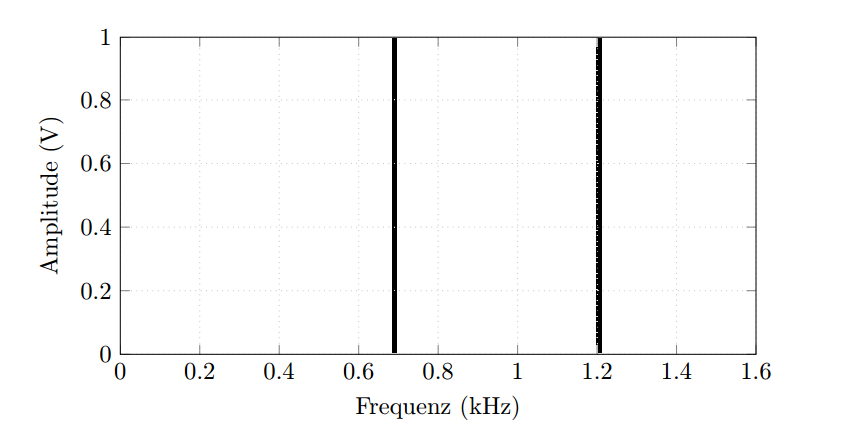
\includegraphics[width=\textwidth]{vorbereitenderBullshit3.png}
              %\caption{Oszilloskop Screenshot}
            \end{figure}
        \end{center}

        \subsection{Sprachsignale}
        \paragraph{Aufgabe}
        In welchem Frequenzbereich liegen Sprach- bzw. Audiosignale? Vergleichen Sie diesen
        Frequenzbereich mit dem Bereich, der beim Mehrfrequenzwahlverfahren belegt wird. Was
        schließen Sie daraus?

        \paragraph{Lösung}
        Sprachsignale liegen ungefähr zwischen $300\si{\hertz}$ und $4\si{k\hertz}$.
        Das heißt, Sprachsignale können die selben Frequenzen wie DTMF-Töne enthalten.
        Um Fehlerkennungen zu vermeiden, sind die DTMF-Frequenzen absichtlich so
        gewählt, dass die Töne dissonant klingen.


        \chapter{Versuchsdurchführung}
        \section{Messung harmonischer Signale}
        \subsection{Einstellung des Oszilloskops}
        \paragraph{Einführung}
        Melden Sie sich zunächst mit ihrem kiz-Account im webvpn an und starten sie die GUI.\@
        Verbinden Sie anschließend den Funktionsgenerator des Oszilloskops über ein BNC Kabel
        mit Kanal 1 des Oszilloskops. Stellen Sie in der GUI für den Funktionsgenerator ein Sinussignal der Frequenz 697 Hz und der Amplitude 1 V ein. Verwenden Sie für die folgenden
        Messungen lediglich die im Oszilloskop integrierten Messfunktionen.

        \subsubsection{Überprüfen der Funktion}
        \paragraph{Aufgabe}
        Überprüfen Sie, ob die von Ihnen gesetzte Einstellungen für den Funktionsgenerator
        der auf dem Schirm des Oszilloskops dargestellten Funktion entsprechen.

        \paragraph{Protokoll}
        \begin{center}
            \begin{figure}[H]
                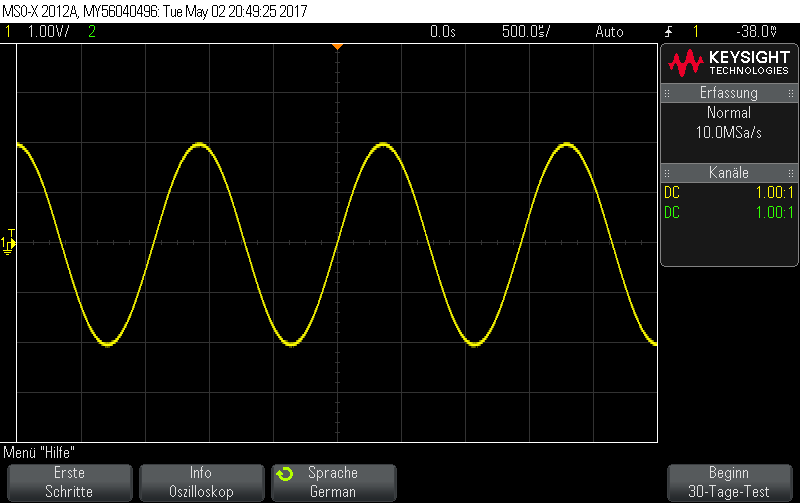
\includegraphics[width=\textwidth]{scope_14.png}
              \caption{Oszilloskop Screenshot}
            \end{figure}
        \end{center}
        Das eingestellte Sinus-Signal wird wie erwartet korrekt dargestellt. Die Amplitude
        beträgt ca. $1\si{\volt}$ und die Frequenz ca. $697\si{\hertz}$.
        \subsubsection{Measure-Funktion}
        \paragraph{Aufgabe}
        Geben Sie die Peak-to-Peak Spannung, den Effektivwert, den Offset und die Frequenz
        des Signals an. Verwenden Sie dazu die \glqq{}Meas.\grqq-{}Funktion und die Cursor des
        Oszilloskops.
        \paragraph{Protokoll}
        \begin{center}
            \begin{figure}[H]
                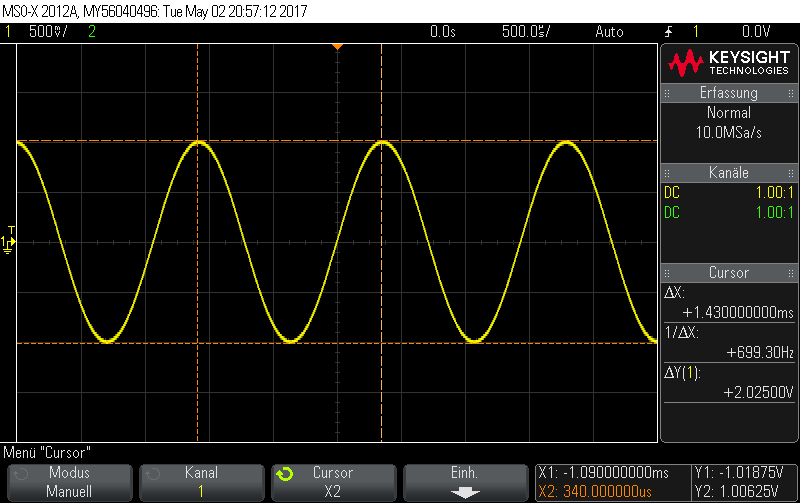
\includegraphics[width=\textwidth]{Screenshot_GUI_4112_cursor.png}
              \caption{Messung mit Cursor}
            \end{figure}
            \begin{figure}[H]
                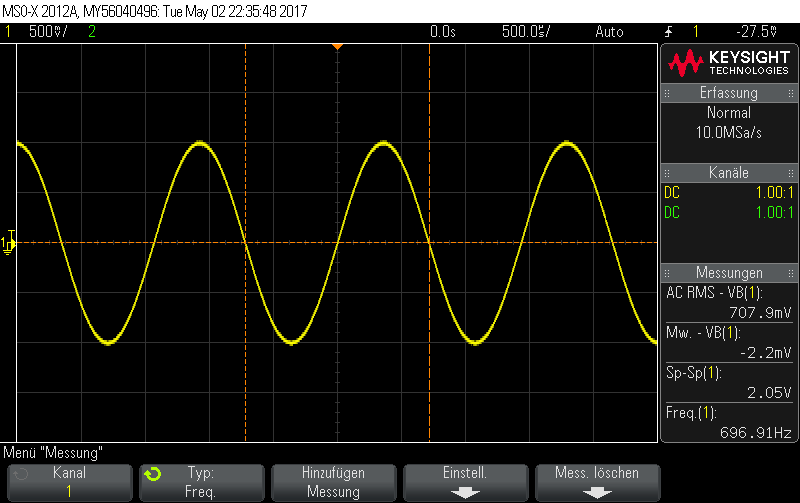
\includegraphics[width=\textwidth]{Screenshot_GUI_4112_Werte.png}
              \caption{Messung mit Measure}
            \end{figure}
            \begin{tabular}{lccccc}
                \toprule
                 & Sollwert & Cursorwert & Measurewert\\
                \midrule
                Peak-to-Peak & $2\si{\volt}$ & $2.025\si{\volt}$ & $2.05\si{\volt}$\\
                Effektivwert & $\frac{1}{\sqrt{2}}\si{\volt} \approx 0.71\si{\volt}$ &  & $707.9\si{m\volt}$\\
                Offset & $0\si{\volt}$ &  & $-2.2\si{m\volt}$\\
                Frequenz & $697\si{\hertz}$ & $699.3\si{\hertz}$ & $696.91\si{\hertz}$ \\
                \bottomrule
            \end{tabular}
        \end{center}


        \vspace{0.5cm}

         Der Effektivwert und das Offset können mit Cursor nicht ohne weiteres
         durch eine Differenz gemessen werden.

        \subsubsection{Plot}
        \paragraph{Aufgabe}
        Stellen Sie die Skalierung der Anzeige über die GUI so ein, dass $5 - 8$ Perioden des
        Signals angezeigt werden und geben Sie die Amplitude des Signals an. Speichern
        Sie den Plot und fügen Sie ihn in das Protokoll ein.
        \paragraph{Protokoll}
        \begin{center}
            \begin{figure}[H]
                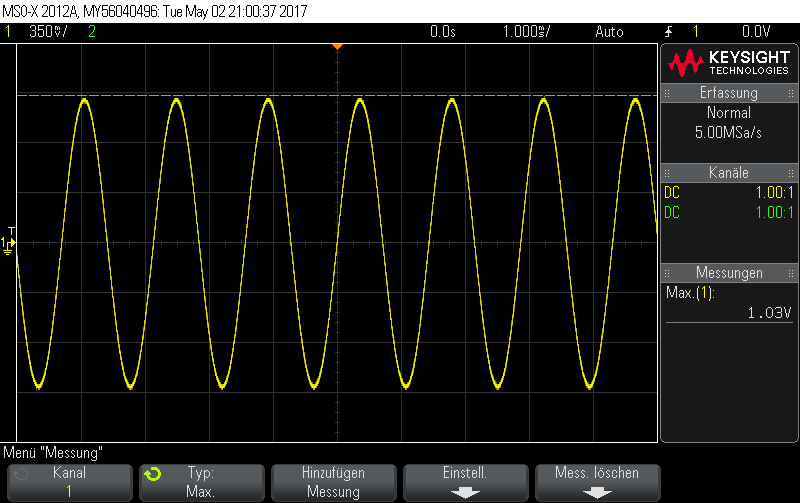
\includegraphics[width=\textwidth]{Screenshot_4113.png}
              \caption{Messung der Amplitude}
            \end{figure}
        \end{center}
        Die Amplitude des Signals beträgt:
        \begin{equation*}
            \hat{U} = 1.03\si{\volt}
        \end{equation*}

        \subsection{Fourier-Transformation}
        %\paragraph{Einführung}
        %Das Oszilloskop verfügt intern über die Möglichkeit die Fourier Transformierte des dargestellten
        %Zeitsignals zu berechnen. Diese soll im Folgenden verwendet werden.
        %Die Auswahl der FFT-Funktion am Oszilloskop erfolgt über
        %\glqq{}Math\grqq{} $\rightarrow$ \glqq{}Operator\grqq{} $\rightarrow$ \glqq{}FFT\grqq{}.
        %Anschließend mussen Spanne und Mittenfrequenz entsprechend des darzustellenden Frequenzbereichs gewählt werden.
        %Unter \glqq{} Mehr FFT\grqq{} lassen sich weitere Einstellungen
        %zur FFT vornehmen: die Fensterfunktion und die vertikale Einheit.
        %Mit Hilfe einer Fensterfunktion lässt sich der sogenannte \glqq{}Leakage effect\grqq{} vermindern.
        %Dieser tritt in der in der digitalen Signalverarbeitung auf, wenn Blocklängen des zu verarbeitenden
        %Signals endlich sind. Hier soll das \glqq{}Hanning-Fenster\grqq{} als Voreinstellung beibehalten
        %werden.
        %Für die vertikale Skalierung gibt es die beiden Möglichkeiten \glqq{}Decibel\grqq{} und
        %\glqq{}$\text{V}_{\text{RMS}}$\grqq{}.
        %In der Einstellung \glqq{}
        %Decibel\grqq{} wird die vertikale Achse logarithmisch aufgetragen, in der
        %Einstellung \glqq{}$\text{V}_{\text{RMS}}$\grqq{} linear. Die Rauschleistung ist in diesem Versuch im Allgemeinen sehr
        %viel kleiner als die Signalleistung. Deshalb ist in der linearen Auftragung mit dem bloßen
        %Auge kein Rauschen sichtbar. Aufgrund dessen wählt man für Spektren in der Regel auch
        %die logarithmische Darstellung, welche im Folgenden auch immer gewählt werden sollte.
        %Die vertikale Einstellung lässt sich nicht über die GUI ändern, diese muss immer händisch
        %am Oszilloskop eingestellt werden.
        \subsubsection{FFT mit dem Oszilloskop}
        \paragraph{Aufgabe}
        Wenden Sie die im Oszilloskop integrierte FFT-Funktion auf das Zeitsignal aus
        Teil 1 an, um das Spektrum zu bestimmen, plotten sie dieses und geben Sie die
        gemessene Frequenz an. Sie können die Einstellungen zur FFT entweder direkt
        am Oszilloskop oder über die GUI vornehmen. Beachten Sie dabei, dass sie den
        dargestellten Frequenzbereich dem Signal entsprechend sinnvoll wählen. Erfassen
        Sie das Spektrum über die GUI und fügen Sie es in das Protokoll ein.
        \paragraph{Protokoll}
        \begin{center}
            \begin{figure}[H]
                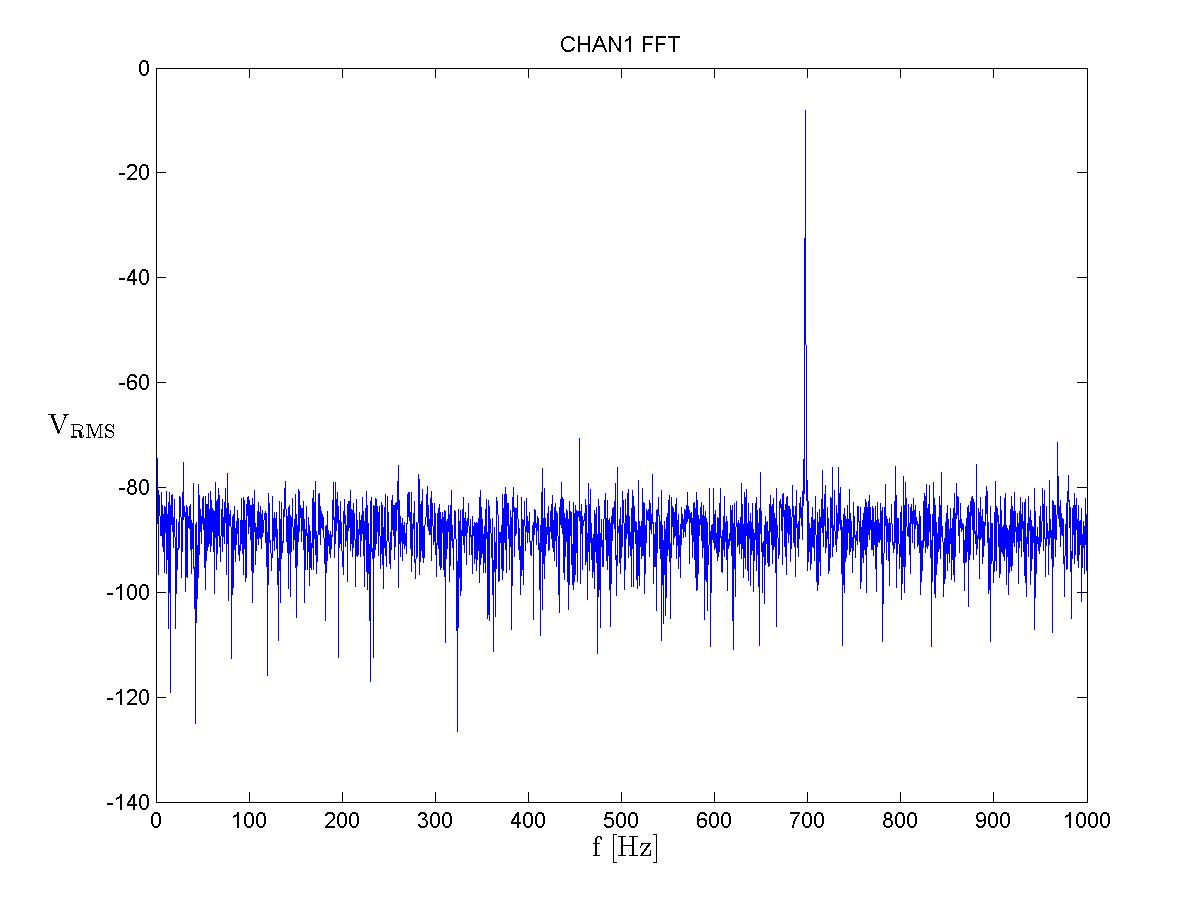
\includegraphics[width=\textwidth]{Screenshot_GUI_4121_chan1_fft.jpg}
              \caption{GUI Screenshot des Frequenzbereichs}
            \end{figure}
        \end{center}

        Die mit durch die FFT bestimmte Frequenz $f_\text{mess} \approx 700\si{\hertz}$
        weicht nur leicht von der erwarteten Frequenz $f_\text{soll} = 697 \si{\hertz}$
        ab.


        \subsubsection{Akustische Ausgabe}
        \paragraph{Aufgabe}
        Das Signal lässt sich am PC akustisch ausgeben. Dazu muss das Zeitsignal mit
        der GUI aufgenommen werden. Wählen Sie dazu im Bereich Measurements Type
        \glqq{}Wave\grqq{} und den entsprechenden Kanal. Über den Button \glqq{}Start\grqq{} wird die Messung
        gestartet. Anschließend kann das Signal in der GUI im Bereich \glqq{}Data\grqq{} ausgewählt
        werden und durch drücken des Button \glqq{}Sound\grqq{} abgespielt werden. Achten Sie darauf,
        dass die Lautstärke in Windows nicht zu leise oder ganz abgeschaltet ist. Hören
        Sie sich das Signal an und beschreiben Sie Ihren Höreindruck.
        \paragraph{Protokoll}
        \begin{center}
            \begin{figure}[H]
                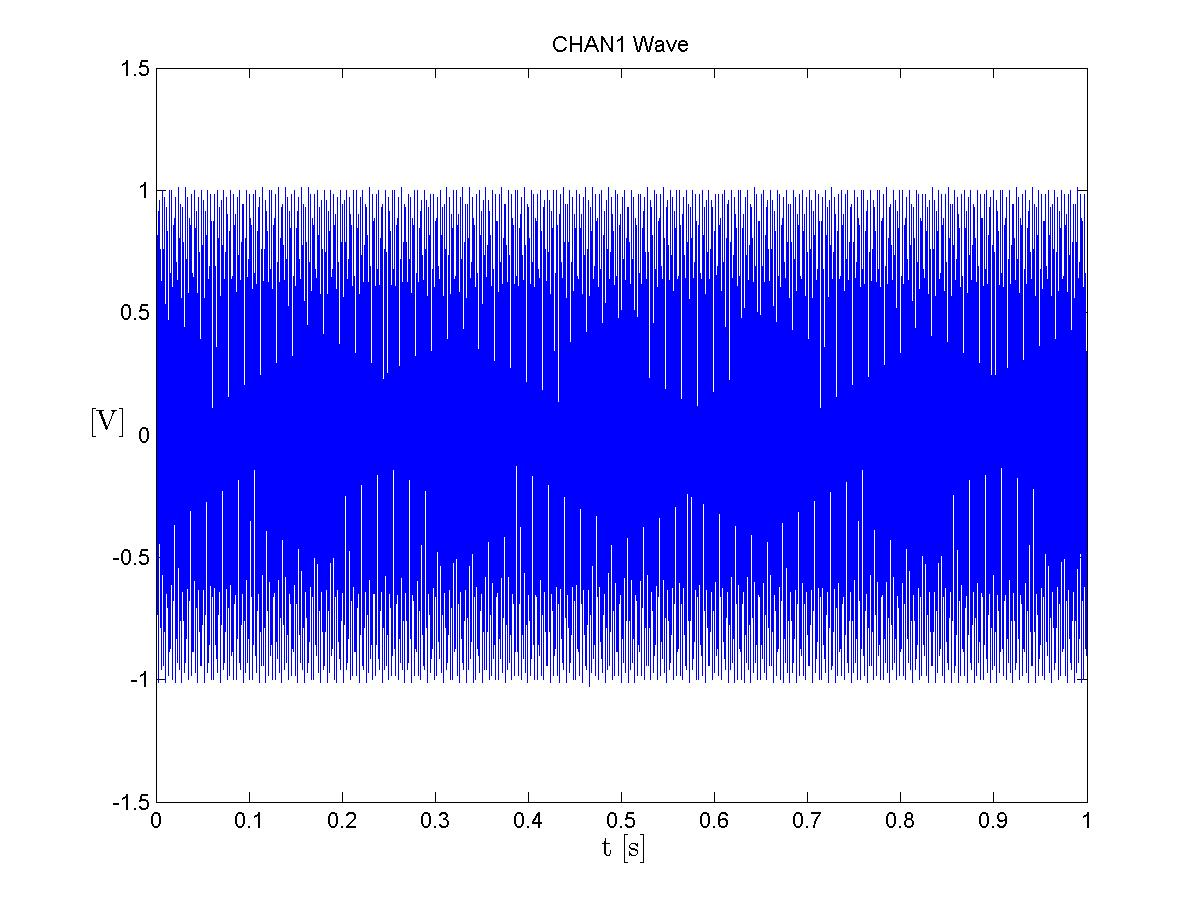
\includegraphics[width=\textwidth]{Screenshot_GUI_4112_Wave_chan1_wave.jpg}
              \caption{Aufgezeichnetes Signal}
            \end{figure}
        \end{center}

        Es ist ein monotoner Sinuston mittlerer Höhe zu hören.

        \subsection{FFT vs. Gehör}
        \paragraph{Aufgabe}
        Stellen Sie am Funktionsgenerator des Oszilloskops unter Verwendung der GUI ein Sinussignal
        der Frequenz $1477\si{\hertz}$ und der Amplitude $1\si{\volt}$ und einem Offset von $100\si{m\volt}$
        ein.

        \subsubsection{Plot}
        \paragraph{Aufgabe}
        Plotten Sie das Signal in Zeit- und Frequenzbereich und geben Sie dabei die Amplitude
        und den Offset bzw.\ die gemessene Frequenz an. Wählen Sie den dargestellten
        Zeitabschnitt so, dass der Signalverlauf erkannt werden kann. Weshalb spielt der
        Offset im Frequenzbereich keine Rolle?
        \paragraph{Protokoll}
        \begin{center}
            \begin{figure}[H]
                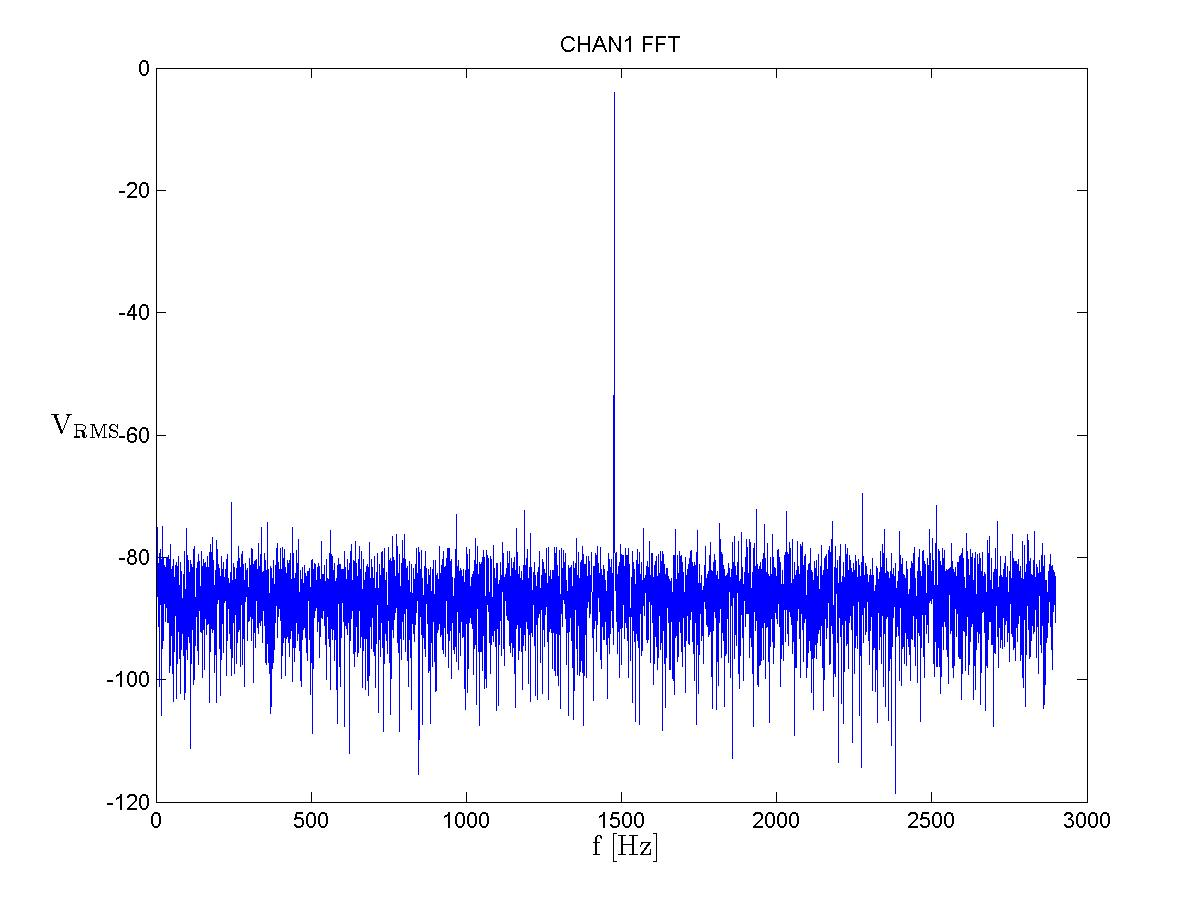
\includegraphics[width=\textwidth]{Screenshot_GUI_4131_FFT_chan1_fft.jpg}
              \caption{GUI Screenshot Frequenzbereich}
            \end{figure}
            \begin{figure}[H]
                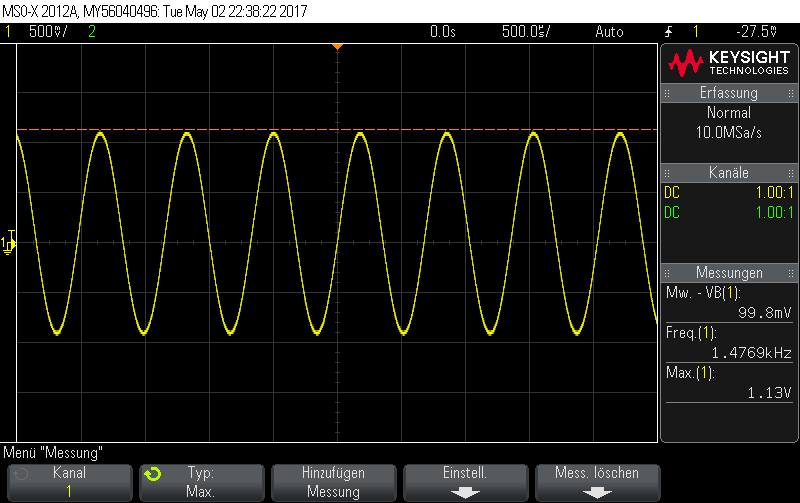
\includegraphics[width=\textwidth]{Screenshot_GUI_4131_Zeit_werte.png}
              \caption{Screenshot  Signalbereich}
            \end{figure}
            \begin{tabular}{lcc}
                \toprule
                & Sollwert & Messwert\\
                \midrule
                Amplitude & $1\si{\volt}$ & $1.03\si{\volt}$\\
                Offset & $100\si{m\volt}$ & $99.8\si{m\volt}$\\
                Frequenz & $1477\si{\hertz}$ & $1476.9\si{\hertz}$\\
                \bottomrule
            \end{tabular}
        \end{center}
        Das Frequenzbild zeigt nur die Amplituden der Teilfrequenzen, ein Offset
        ändert diese nicht, da das Offset eine Frequenz von $0\si{\hertz}$ hat.
        Theoretisch müsste man bei $0 \si{\hertz}$ erkennen. Da das Offset jedoch
        nur $100 \si{m\volt}$ beträgt und somit unter der 3dB Grenzfrequenz liegt
        und weiterhin im Rauschen untergeht, lässt sich der Peak nicht erkennen.

        \subsubsection{Höreindruck}
        \paragraph{Aufgabe}
        Hören Sie sich das Signal an und vergleichen Sie den Höreindruck mit dem zuvor
        abgespielten Signal.
        \paragraph{Protokoll}
        \begin{center}
            \begin{figure}[H]
                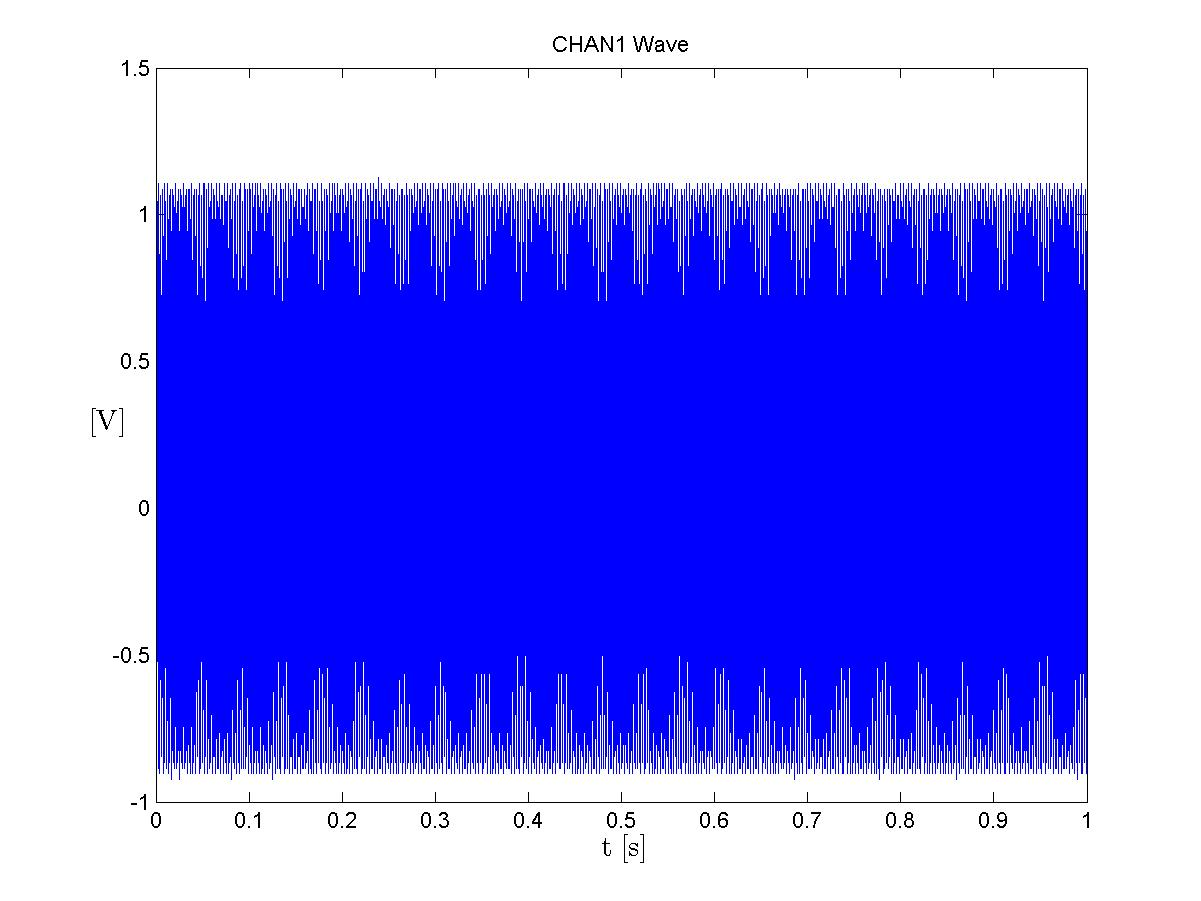
\includegraphics[width=\textwidth]{Screenshot_GUI_4132_chan1_wave.jpg}
              \caption{Aufgezeichnetes Signal}
            \end{figure}
        \end{center}

        Das Ton ist, wie zu erwarten, deutlich höher als der erste Ton, weist aber
        die gleichen monotonen Charakteristiken auf.

        \subsubsection{Höreindruck bei kleinen Frequenz-Differenzen}
        \paragraph{Aufgabe}
        Stellen Sie nun ein Signal der Frequenz $1480\si{\hertz}$ und der Amplitude $1\si{\volt}$ am Funktionsgenerator
        ein und hören Sie sich auch dieses Signal an. Können die beiden
        Signale mit Frequenzen von $1477\si{\hertz}$ und $1480\si{\hertz}$ akustisch voneinander unterschieden
        werden? Wenn nicht, weshalb ist dies nicht möglich?
        \paragraph{Protokoll}

        Das menschliche Gehör verfügt nicht über die Möglichkeit, Frequenzunterschiede
        von $3 \si{\hertz}$ aufzulösen.

        \subsubsection{Auflösung}
        \paragraph{Auflösung}
        Wie groß muss dass Messintervall gewählt werden, damit diese beiden Signale
        mittels FFT unterschieden werden können? Wie vielen Perioden des Signals mit
        $1480\si{\hertz}$ entspricht dies?
        \paragraph{Protokoll}

        \begin{eqnarray*}
            f_{Aufloesung} &=& \frac{1}{N \cdot T}\\
            T &=& \frac{1}{f}\\
            f_{Aufloesung} &=& 3 \si{\hertz}\\
            \Rightarrow N &=& \frac{1}{f_{Aufloesung} \cdot T} = \frac{1}{3 \si{\hertz} \cdot \frac{1}{1480\si{\hertz}}} \approx 494\\
            T_{Mess} &=& \frac{1}{f} \cdot N = 0.33 \si{\second}
        \end{eqnarray*}

        Um eine Frequenzauflösung von $3\si{\hertz}$ zu erreichen, müssen mindestens
        494 Perioden aufgezeichnet werden. Das entspricht ungefähr $\frac{1}{3} \si{\second}$.

        \section{Messung periodischer Signale}
        %\paragraph{Einführung}
        %Verbinden Sie den Eingang des externen Trigges am Oszilloskop (auf der Rückseite) und
        %den \glqq{}TTL/CMOS OUTPUT\grqq{} des externen Funktionsgenerators mit einem BNC Kabel.
        %Bei einigen Funktionsgeneratoren muss der \glqq{}SYNC Out\grqq{} gewählt werden. Stellen Sie
        %anschließend den Trigger des Oszilloskops auf \glqq{}extern\grqq{} ein. Das Oszilloskop wird nun auf
        %das Signal des externen Frequenzgenerators getriggert.
        %Im Folgenden werden ein Signal des externen und ein Signal des internen Funktionsgenerators
        %über ein T-Stück addiert und auf Kanal 1 geführt.
        %Verbinden Sie dazu den Ausgang des externen Funktionsgenerators über die eine Seite
        %des T-Stücks mit Kanal 1 des Oszilloskops. Stellen Sie nun ein Sinussignal der Frequenz
        %697 Hz ein. VSS soll dabei etwa 2 V betragen. Überprüfen Sie die Amplitude des Signals
        %auf dem Schirm des Oszilloskops.
        %Stellen Sie am Funktionsgenerator des Oszilloskops ein Signal der Frequenz 1336 Hz,
        %Amplitude 1 V und Offset 0 V ein. Addieren Sie die beiden Signale unter Verwendung des
        %T-Stücks indem Sie das Ausgangssignal des Funktionsgenerators des Oszilloskops über
        %ein BNC-Kabel auf das zweite Ende des T-Stücks geben.

        \subsubsection{Stehende Welle}
        \paragraph{Aufgabe}
        Wieso erhält man keine stehende Welle auf dem Schirm des Oszilloskops? Weshalb
        spielt das bei der Berechnung der FFT keine Rolle?
        \paragraph{Protokoll}
        Die Messung wird durch den externen Trigger getriggert, da das zweite Signal
        eine andere Frequenz als das Trigger-Signal hat, ist die Phase zum ersten Signal
        bei jeder Messung anders und es wird kein stehendes Bild auf dem Oszilloskop
        abgebildet.

        Die FFT zerlegt lediglich das Summensignal in die einzelnen Frequenzteile,
        dabei wird in immer gleichen Zeitabständen gemessen. Ein Summensignal aus
        mehreren Frequenzen ist deshalb unproblematisch.

        \subsubsection{Plot}
        \paragraph{Aufgabe}
        Plotten Sie einen geeigneten Ausschnitt des Summensignals im Zeitbereich. Geben
        Sie den Minimal- und Maximalwert des Signals an.
        \paragraph{Protokoll}
        \begin{center}
            \begin{figure}[H]
                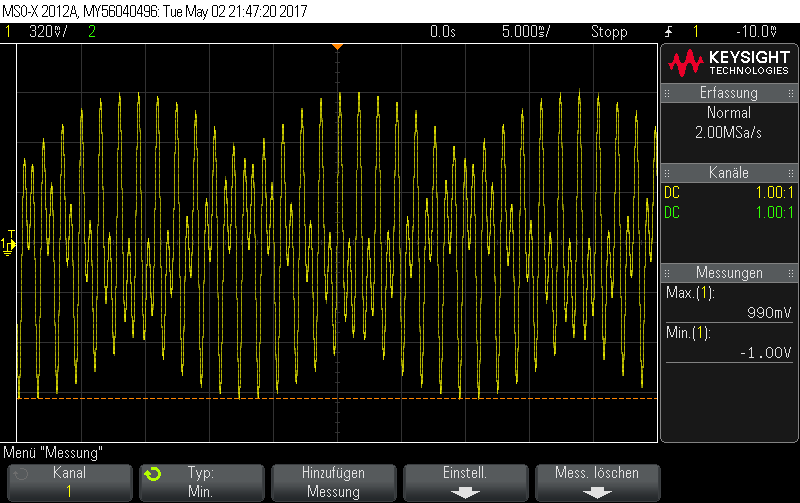
\includegraphics[width=\textwidth]{Screenshot_GUI_4202.png}
              \caption{Summensignal im Zeitbereich}
            \end{figure}
        \end{center}

        \begin{eqnarray*}
            U_{\min{}} &=& -1.00\si{\volt}\\
            U_{\max{}} &=& 990\si{m\volt}
        \end{eqnarray*}

        \subsubsection{Höreindruck}
        \paragraph{Aufgabe}
        Hören Sie sich einen geeigneten Zeitausschnitt des Summensignals mit Hilfe der
        \glqq{}Sound\grqq{}-Funktion an und beschreiben Sie den Höreindruck.
        \paragraph{Protokoll}
        Die Überlagerung der beiden Frequenzen klingt dissonant. Es fällt auf, dass
        der Wahlton für die Taste 2 identisch klingt. Dies lässt sich durch
        Betrachten der Grafik \ref{fig:DTFM_PAD} erklären.


        \subsubsection{Frequenzbereich}
        \paragraph{Aufgabe}
        Transformieren Sie das Signal in den Frequenzbereich und plotten Sie es. Geben Sie
        die auftretenden Frequenzen an.
        \paragraph{Protokoll}
        \begin{center}
            \begin{figure}[H]
                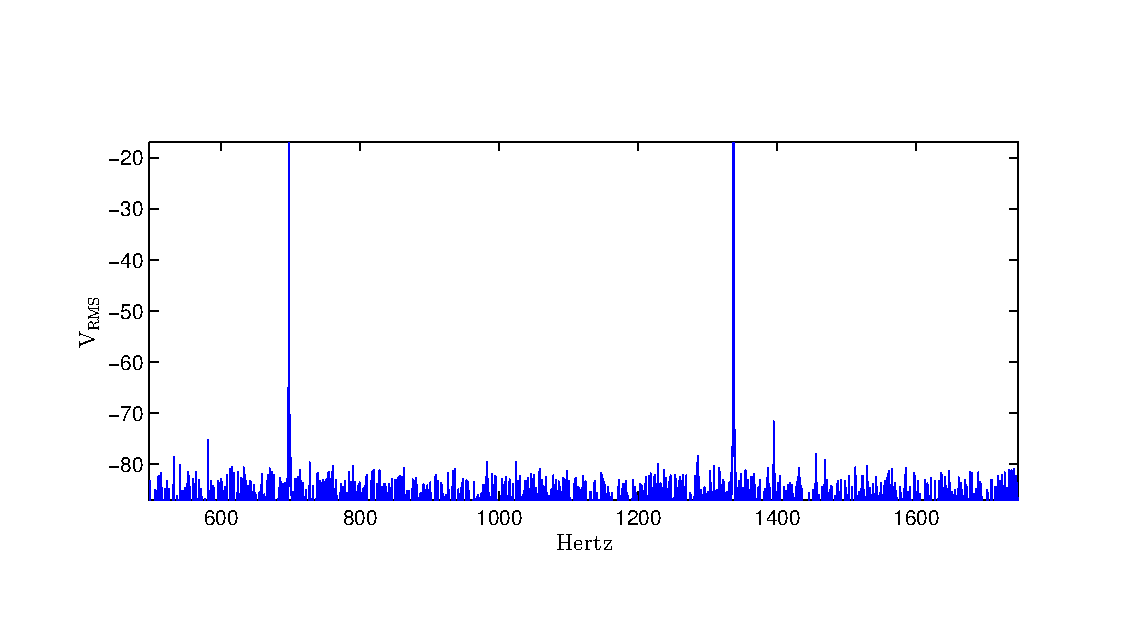
\includegraphics[width=\textwidth]{Screenshot_GUI_4204_beser}
              \caption{Summensignal im Frequenzbereich}
            \end{figure}
        \end{center}
        \begin{eqnarray*}
            f_1 &\approx& 700\si{\hertz}\\
            f_2 &\approx& 1400\si{\hertz}
        \end{eqnarray*}

        Im Frequenzbereich lassen sich zwei Peaks erkennen: bei ca. $700\si{\hertz}$
        und bei ca. $1400\si{\hertz}$. Diese entsprechen den eingestellten
        Frequenzen.

        \subsubsection{Bandbreite}
        \paragraph{Aufgabe}
        Geben Sie die Bandbreite sowie die obere und untere Grenzfrequenz des Signals an.
        \paragraph{Protokoll}
        Die angebenen Frequenzen sind die beiden Grenzfrequenzen, alle anderen
        Peaks sind weit unterhalb der $3$dB Grenzfrequenz, und damit für die
        Bandbreitenbestimmung irrelevant.

        Die Bandbreite ergibt sich aus der Differenz der beiden Grenzfrequenzen
        und beträgt ca. $700\si{\hertz}$.
        \begin{eqnarray*}
            f_1 &\approx& 700\si{\hertz}\\
            f_2 &\approx& 1400\si{\hertz}\\
            B &=& f_2 - f_1 = 700\si{\hertz}
        \end{eqnarray*}

        \section{Mehrfrequenzwahlverfahren}
        \begin{center}
            \begin{figure}[H]
                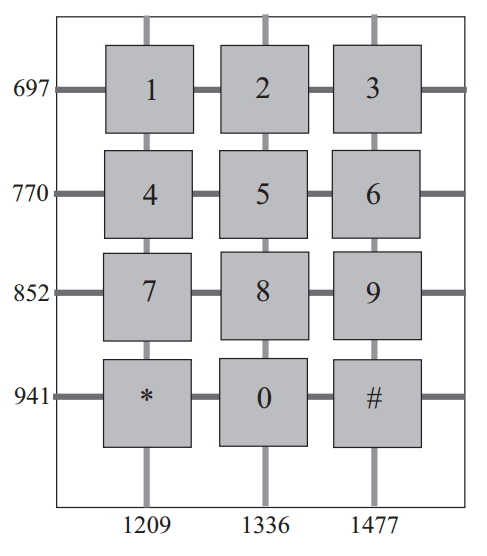
\includegraphics[width=\textwidth]{dtmf_pad.jpg}
                \caption{DTMF Tasten}
                \label{fig:DTFM_PAD}
            \end{figure}
        \end{center}
        \subsection{DTMF-App}
        \paragraph{Aufgabe}
        Für diesen Versuchsteil benötigen Sie nun die zuvor auf Ihr Mobiltelefon geladene \glqq{}DTMF\grqq{} App.
        Verbinden Sie den Kopfhörerausgang Ihres Mobiltelefons mit einem 3.5 mm Klinke-Kabel
        über das Steckbrett mit Kanal 1 des Oszilloskops. Parallel dazu schalten Sie einen Kopfhörer.

        Schauen Sie sich die Frequenzen einzelner Töne mit der Fourier-Transformation auf dem
        Oszilloskop an. Beschreiben Sie Ihren Höreindruck sowie Ihre Beobachtungen auf dem
        Oszilloskop bei einer waagrechten, senkrechten und diagonalen Tastenfolge.
        \paragraph{Protokoll}
        \begin{center}
            \begin{figure}[H]
                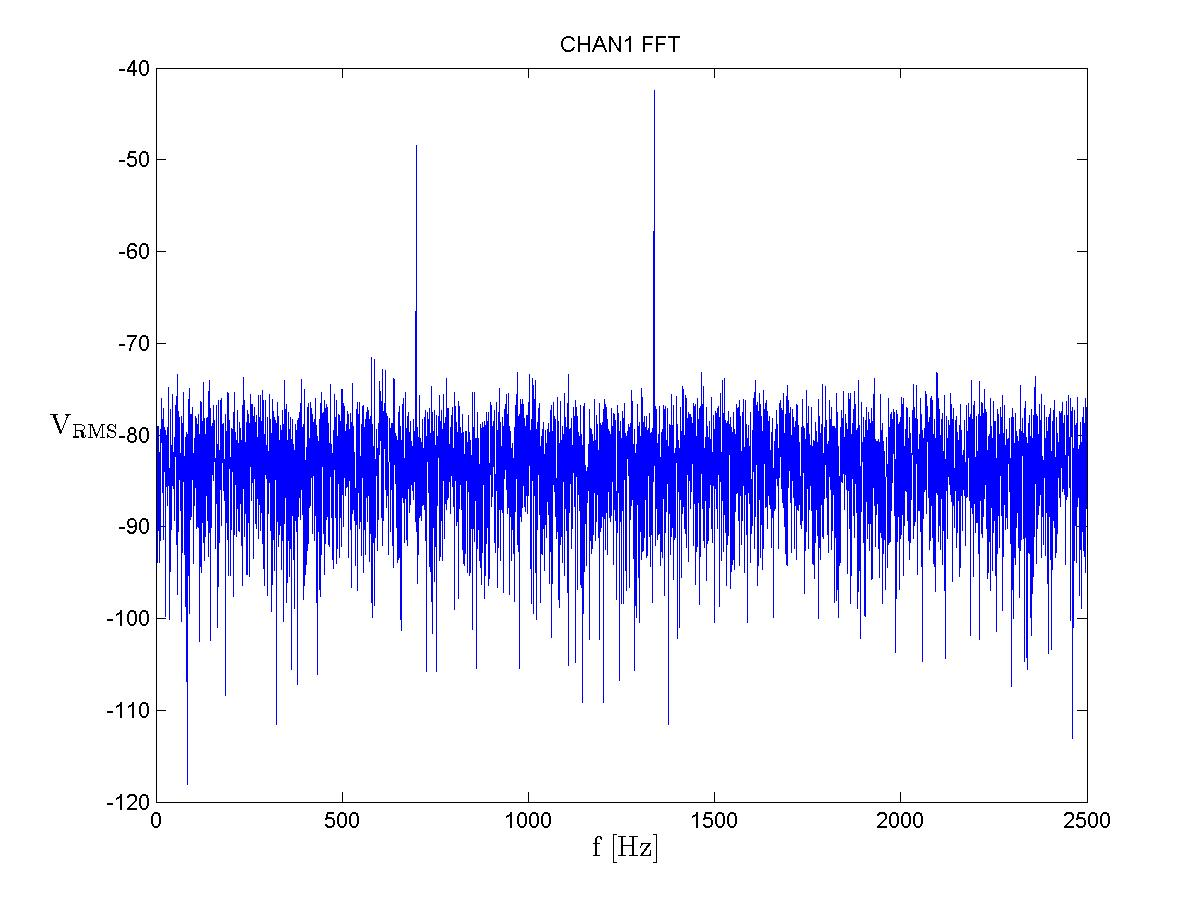
\includegraphics[width=\textwidth]{Screenshot_GUI_431_T2_chan1_fft.jpg}
                \caption{Frequenzbild für Taste 2}
            \end{figure}
            \begin{figure}[H]
                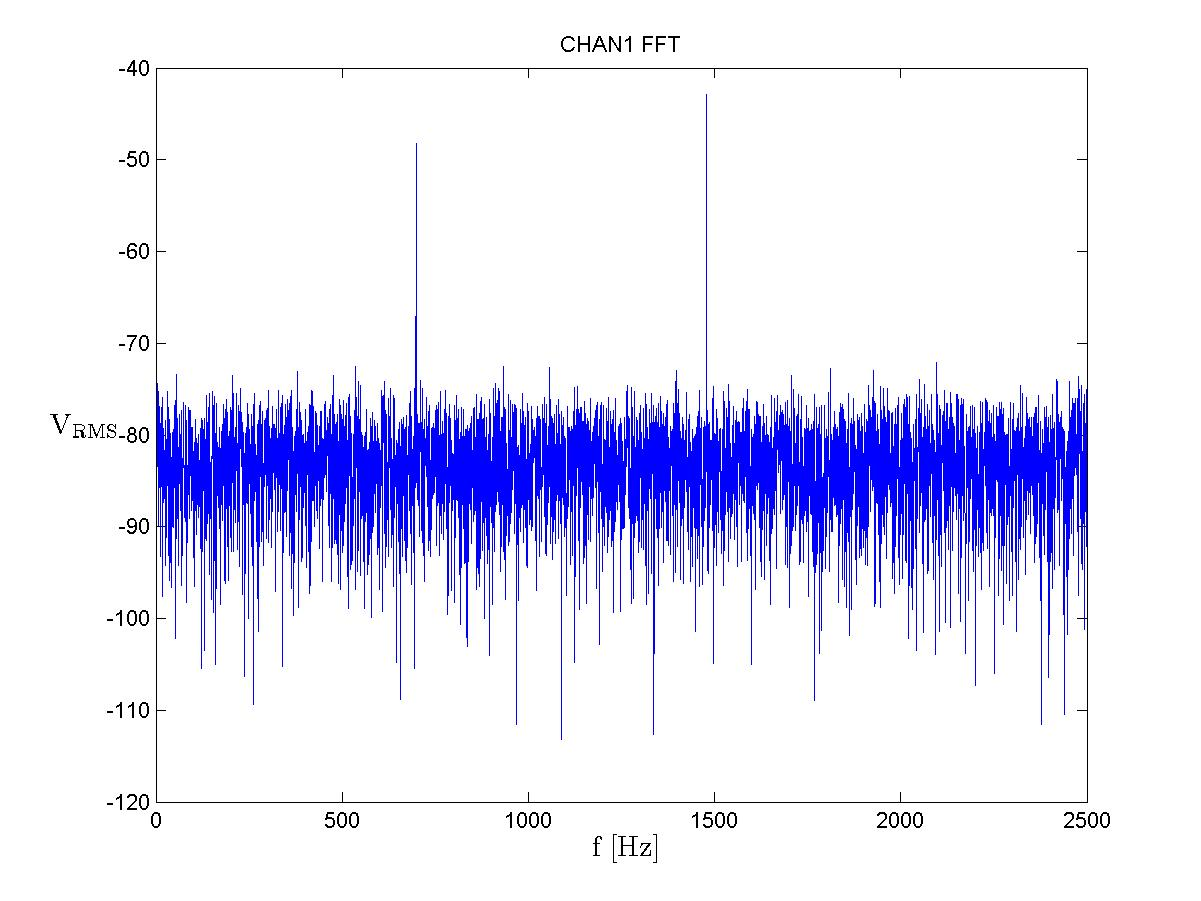
\includegraphics[width=\textwidth]{Screenshot_GUI_431_T3_chan1_fft.jpg}
                \caption{Frequenzbild für Taste 3}
            \end{figure}
            \begin{figure}[H]
                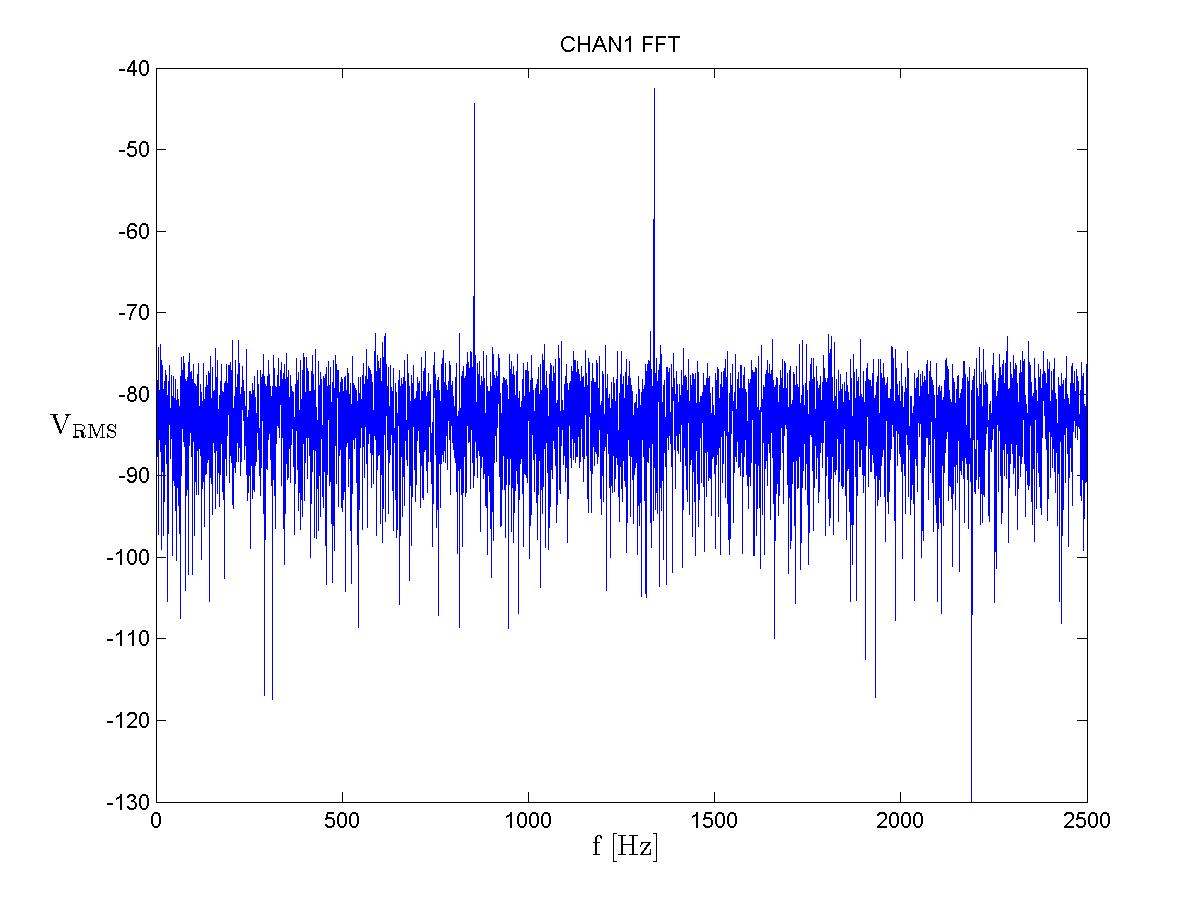
\includegraphics[width=\textwidth]{Screenshot_GUI_431_T8_chan1_fft.jpg}
                \caption{Frequenzbild für Taste 8}
            \end{figure}
        \end{center}
        Bei jeder Taste ist ein dissonanter Ton zu hören. Bei unterschiedlichen Tasten
        in gleicher Reihe oder Spalte ändert sich jeweils einer der beiden überlagerten
        Töne.

        Aus den Diagrammen lässt sich folgern, dass durch eine Bewegung in der x-Achse
        (zum Beispiel von Taste 2 auf Taste 3) die obere Grenzfrequenz verschoben wird. Eine Ziffer weiter
        rechts bewirkt eine höhere obere Grenzfrequenz.
        Bewegt man sich in der y-Achse (zum Beispiel von Taste 2 auf Taste 8)
        verschiebt sich die untere Grenzfrequenz. Hier bedeutet eine Bewegung
        nach unten eine höhere untere Grenzfrequenz.
        Bei einer diagonalen Bewegung (zum Beispiel von Taste 3 auf Taste 8) ändern
        sich folglich beide Grenzfrequenzen.

        \subsection{Matlab}
        %\paragraph{Einführung}
        %Im Folgenden sollen die zuvor durch die beiden Funktionsgeneratoren realisierten Oszillatoren
        %in MATLAB umgesetzt werden. Dadurch sollen zunächst einige Töne, wie sie
        %beim Mehrfrequezwahlverfahren verwendet werden synthetisiert und im abschließenden
        %Versuchsteil eine \glqq{}gewählte\grqq{} Telefonnummer unter Verwendung der FFT analysiert werden.
        %Oszilloskop, BNC Kabel und Frequenzgenerator werden in diesem Versuchsteil nicht
        %mehr benötigt.
        %Laden Sie sich das Archiv \texttt{DTMF\_Student.zip} von der Praktikumsseite herunter und
        %entpacken Sie es. Wechseln Sie anschließend innerhalb von MATLAB in den Ordner mit
        %den entpackten Dateien. Hier finden Sie folgenden MATLAB Files:
        %\begin{itemize}
        %    \item \texttt{dial\_tones.m}
        %
        %        Spielt die vom Benutzer gewählte Nummer ab und plottet die DTMF-Töne in Zeit-
        %        und Frequenzbereich. Zwischen den einzelnen Ziffern wird dabei eine Pause der
        %    \item \texttt{dialed\_number.mat}
%
%                MATLAB Stuct, mit der zu analysierenden Nummer. Zur Weiteren Verabeitung
%                muss das Struct zunächst in MATLAB importiert werden. Dies kann über einen
%                Rechtsklick auf das File ausgewählt werden.
%
%            \item \texttt{dtmfcut.m}
%
%                Wird verwendet um die gesendete Nummer in einzelne Zeitabschnitte zu zerlegen
%                und die Fourier Transformierte über diese einzelnen Zeitabschnitte zu berechnen.
%                Der Aufruf erfolgt automatisch innerhalb der Funktion \texttt{receive\_dial}.
%
%            \item \texttt{fft\_dtmf.m}
%                Diese Funktion enthält ein Codefragment das während dieses Praktikumsversuchs
%                vervollständigt werden soll um die gespeicherte Telefonnummer in Zeit- und Fre-
%                quenzbereich zu plotten und anhören zu können.
%
%            \item \texttt{generate\_tones.m}
%
%                Erzeugt die entsprechenden DTMF Töne, wenn eine Taste entsprechend der Tastenbelegung aus Abbildung 10 gewählt wird. Die Eingabe muss dabei nach der
%                Eingabeaufforderung als String erfolgen. Diese Funktion enthält einige Lücken und muss während des Versuchs
%                vervollständigt werden.
%
%            \item \texttt{receive\_dial.m}
%
%                Gibt die gewählte Telefonnummer zurück, indem das gewählte Signal mittels FFT
%                analysiert wird. Zusätzlich wird jede einzelne erkannte Ziffer in Zeit und Frequenz-
%                bereich geplottet.
%        \end{itemize}

        \subsection{Sourcecode}
        \paragraph{Aufgabe}
        In der Datei \texttt{generate\_tones.m} fehlen einige Zeilen. Vervollständigen Sie den Code. Die
        Korrektheit des Codes kann durch Aufruf der Funktion \texttt{dial\_tones.m} überprüft werden.
        (Eingabe von \texttt{dial\_tones();} im Commandwindow und in der Eingabeaufforderung dann
        beispielsweise ’2’, achten sie auf die Hochkommata).
        \paragraph{Protokoll}
        Vervollständigter Code:
        \lstinputlisting[language=Matlab, firstline=10, lastline=19]{generate_tones_Student.m}

        \vspace{2cm}

        \lstinputlisting[language=Matlab, firstline=85, lastline=92]{generate_tones_Student.m}

        \subsection{FFT Tastentöne}
        \subsubsection{Plots des Mehrfrequenzverfahrens}
        \paragraph{Aufgabe}
        Verwenden Sie die Funktion \texttt{dial\_tones} um das Signal für die Taste
        \glqq{}1\grqq{} im Mehrfrequenzwahlverfahren
        zu erzeugen und hören Sie es sich an. Geben Sie die auftretenden
        Frequenzen an und fügen Sie die beiden Plots in das Protokoll ein. Skalieren
        Sie die Diagramme dafür sinnvoll.
        \paragraph{Protokoll}
        \begin{center}
            \begin{figure}[H]
                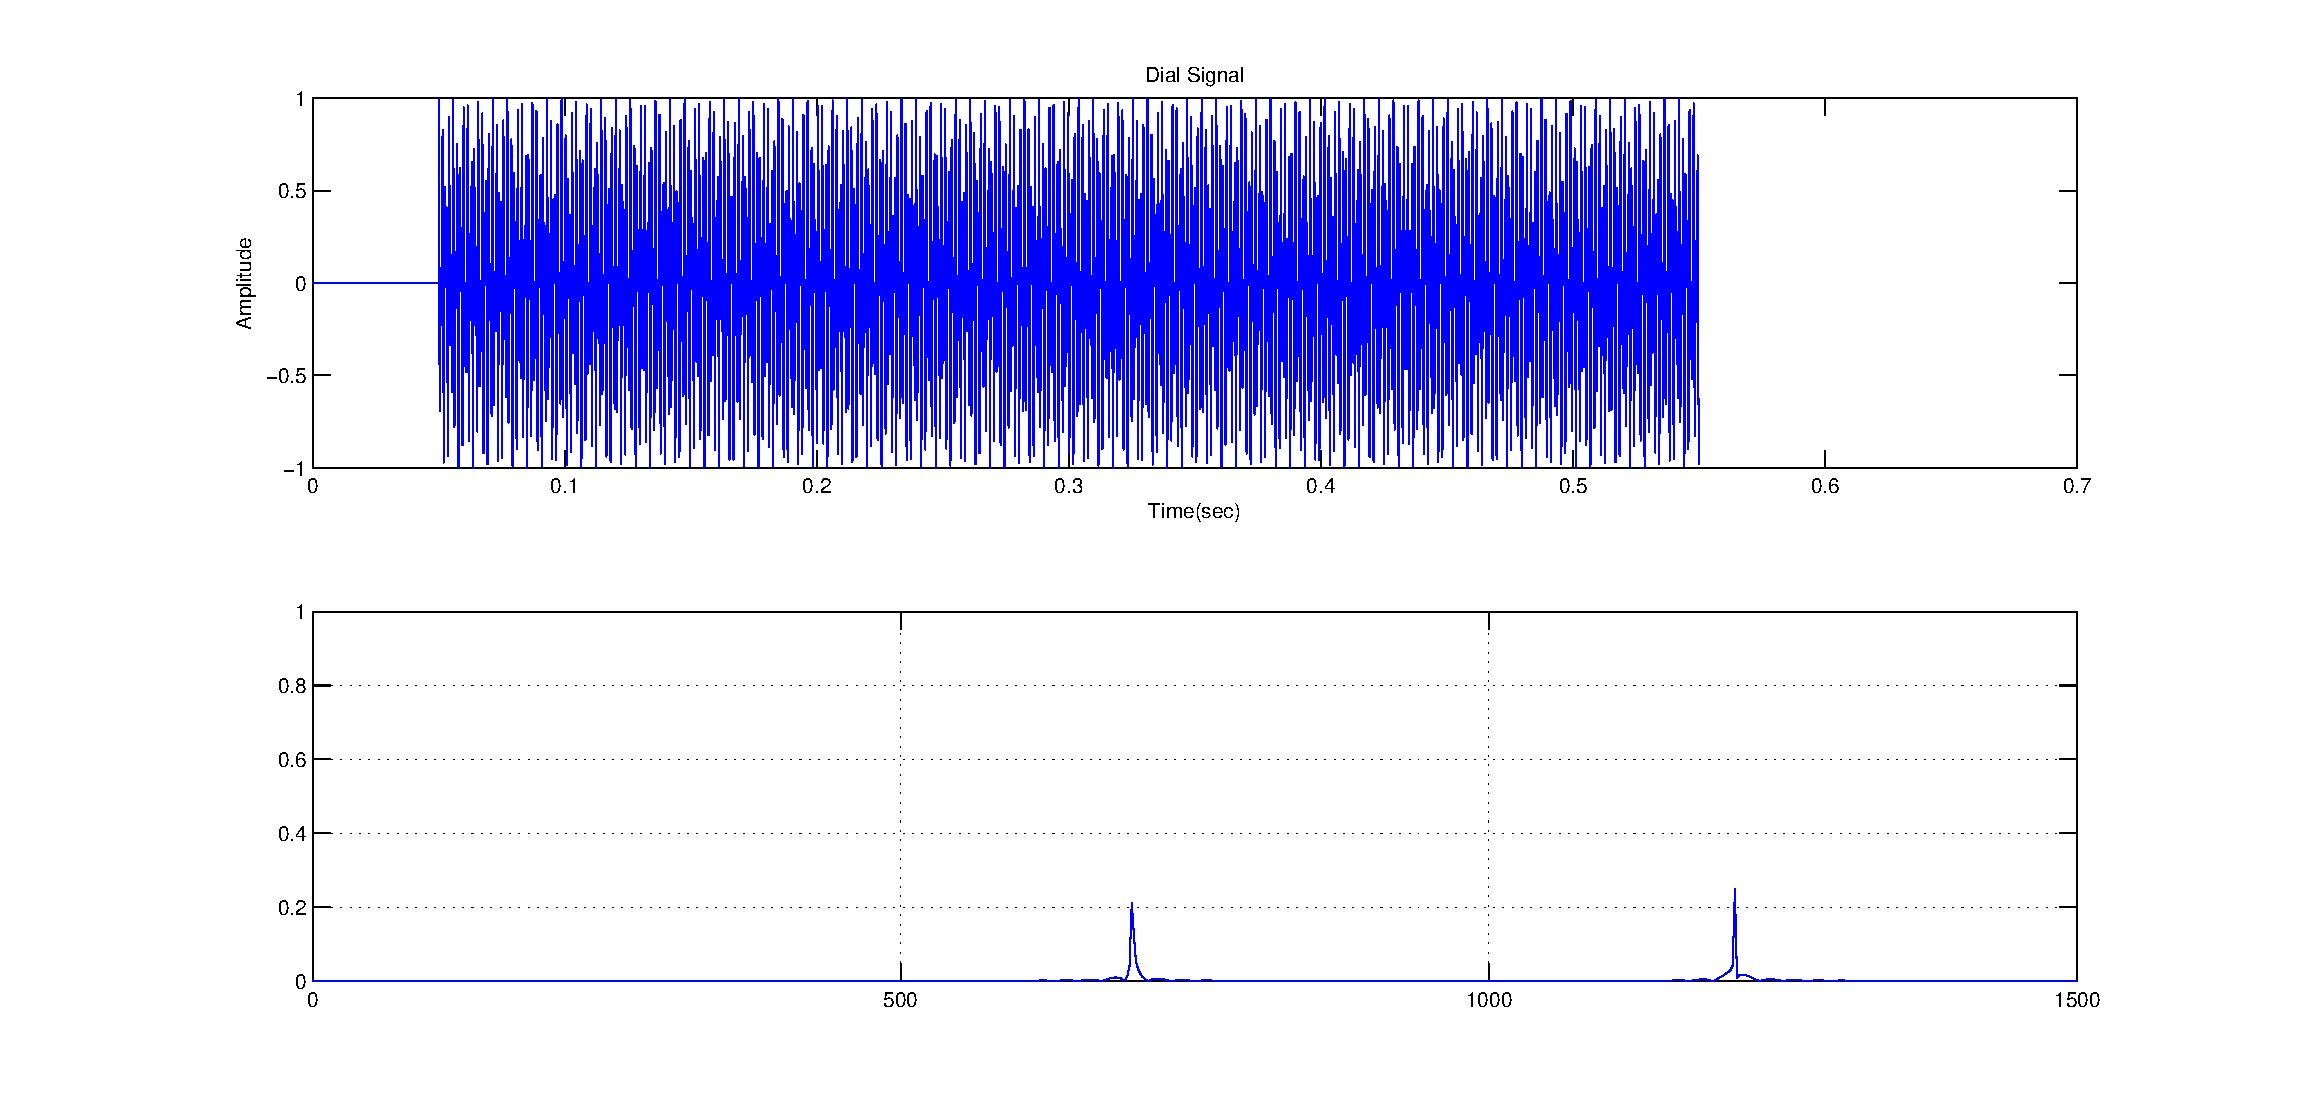
\includegraphics[width=\textwidth]{img4341}
              \caption{\texttt{dial\_tones} mit Eingabe \texttt{1}}
            \end{figure}
        \end{center}
        Auftretende Frequenzen:
        \begin{eqnarray*}
            f_{1_{fft}} &=& 696.38 \si{\hertz}\\
            f_{1_{soll}} &=& 697\si{\hertz}\\
            f_{2_{fft}} &=& 1209.12\si{\hertz}\\
            f_{2_{soll}} &=& 1209\si{\hertz}
        \end{eqnarray*}
        Die zwei zu erkennenden Peaks lassen sich eindeutig einer Ziffer zuordnen.

        Die geringe Abweichung zur jeweils eingestellten Frequenz ist der Umrechnung
        vom Frequenzbereich zum Bildbereich und wieder zurück geschuldet.

        \subsubsection{Tastentöne}
        \paragraph{Aufgabe}
        Hören Sie sich 2 weitere beliebige Tastentöne an und analysieren Sie die Signale im
        Frequenzbereich. Verwenden Sie dazu erneut die Funktion \texttt{dial\_tones} und wählen
        Sie jeweils nur eine Ziffer auf einmal.
        \paragraph{Protokoll}

        \begin{center}
            \begin{figure}[H]
                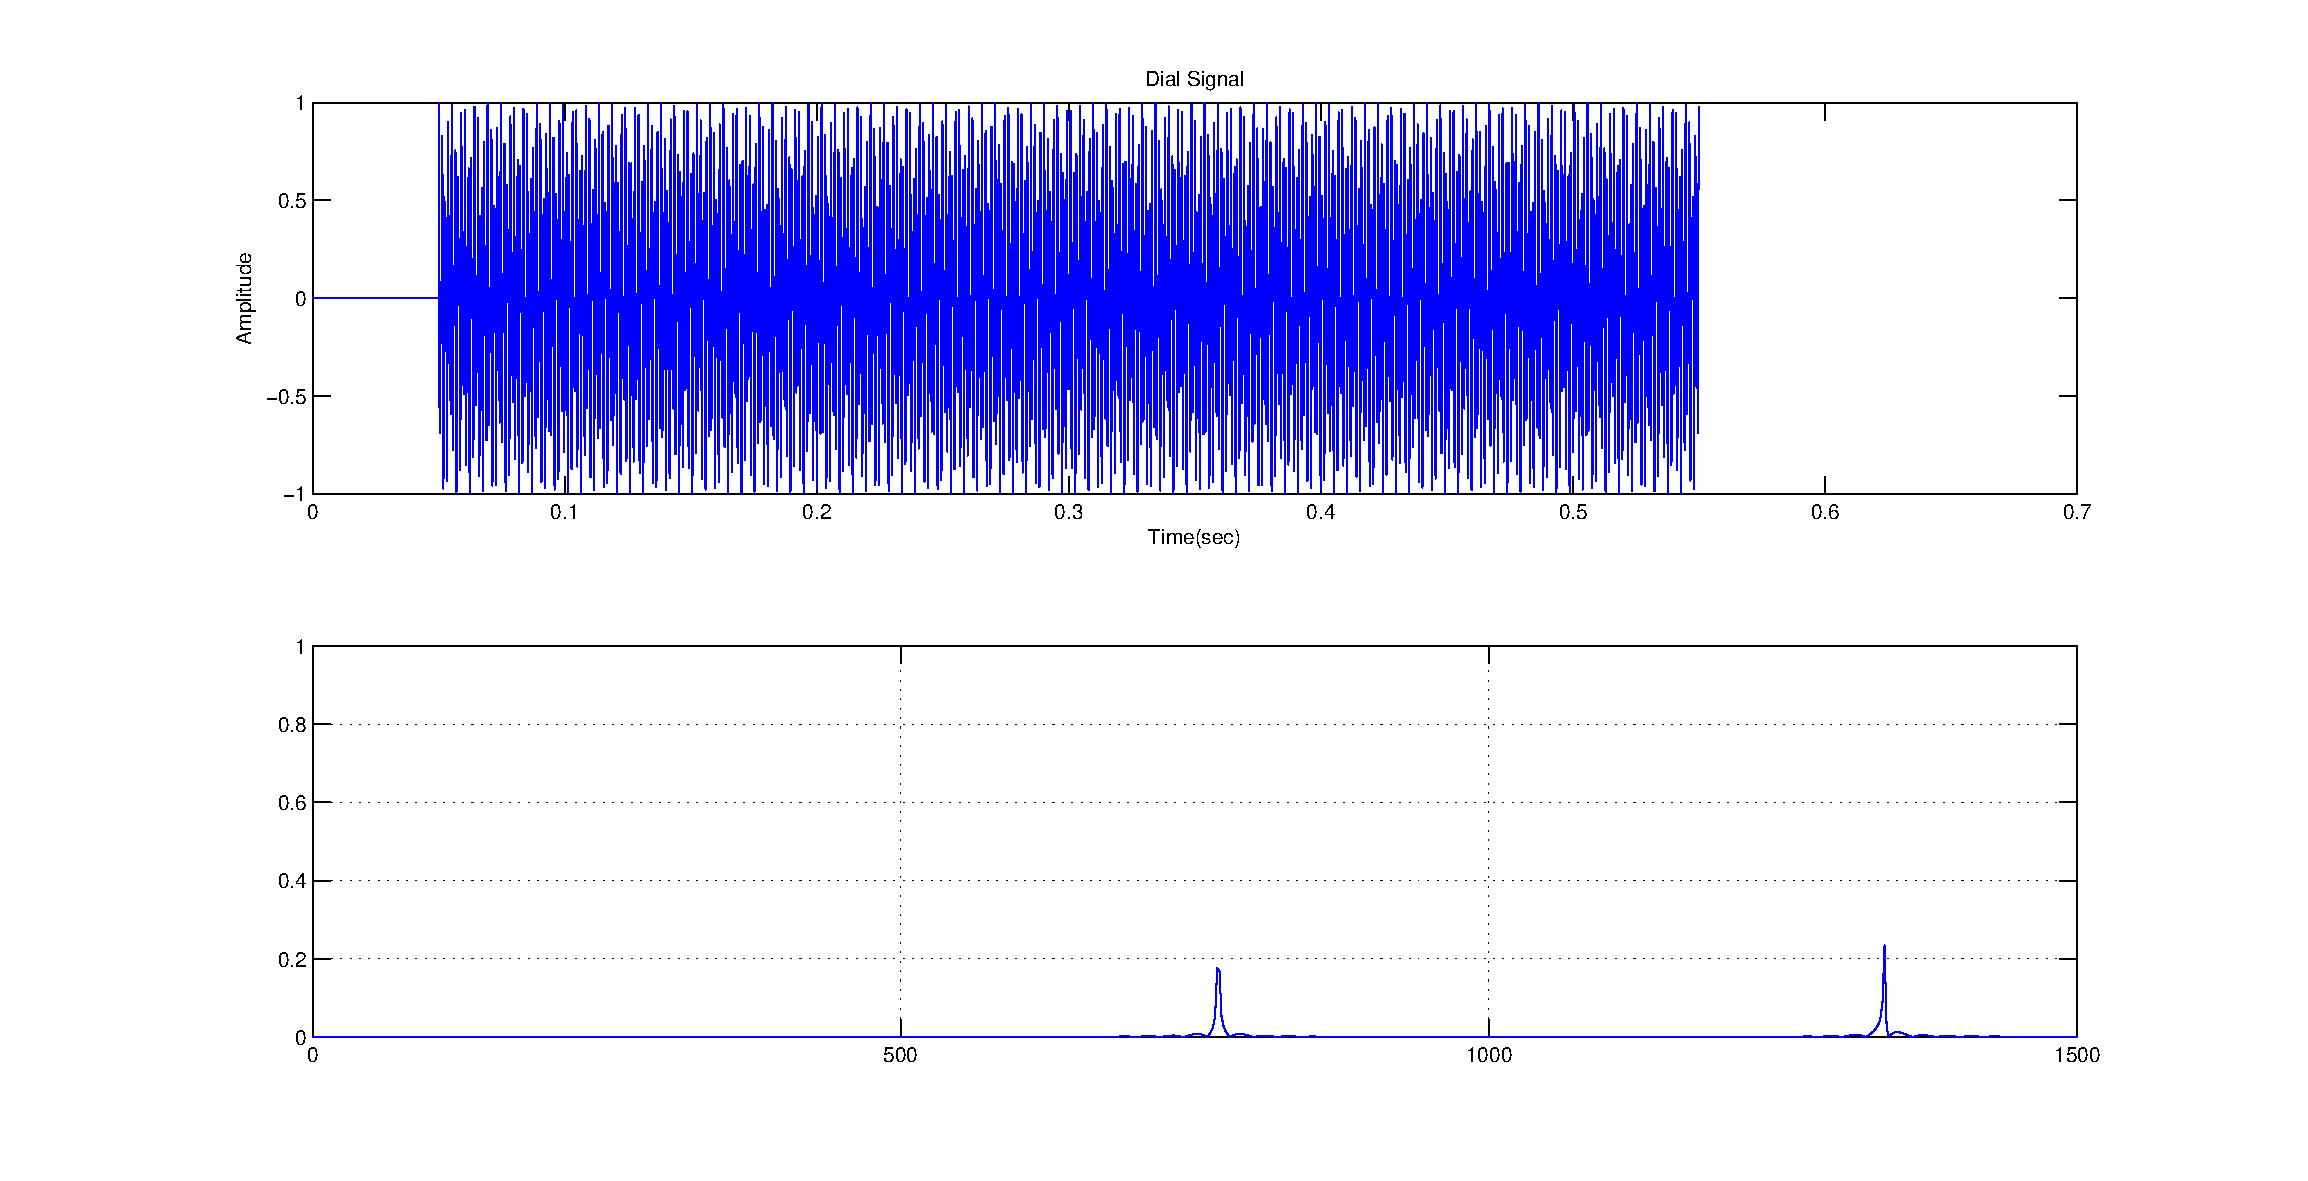
\includegraphics[width=\textwidth]{img43421}
                \caption{\texttt{dial\_tones} mit Eingabe \texttt{5}, ohne Zoom}
            \end{figure}
            \begin{figure}[H]
                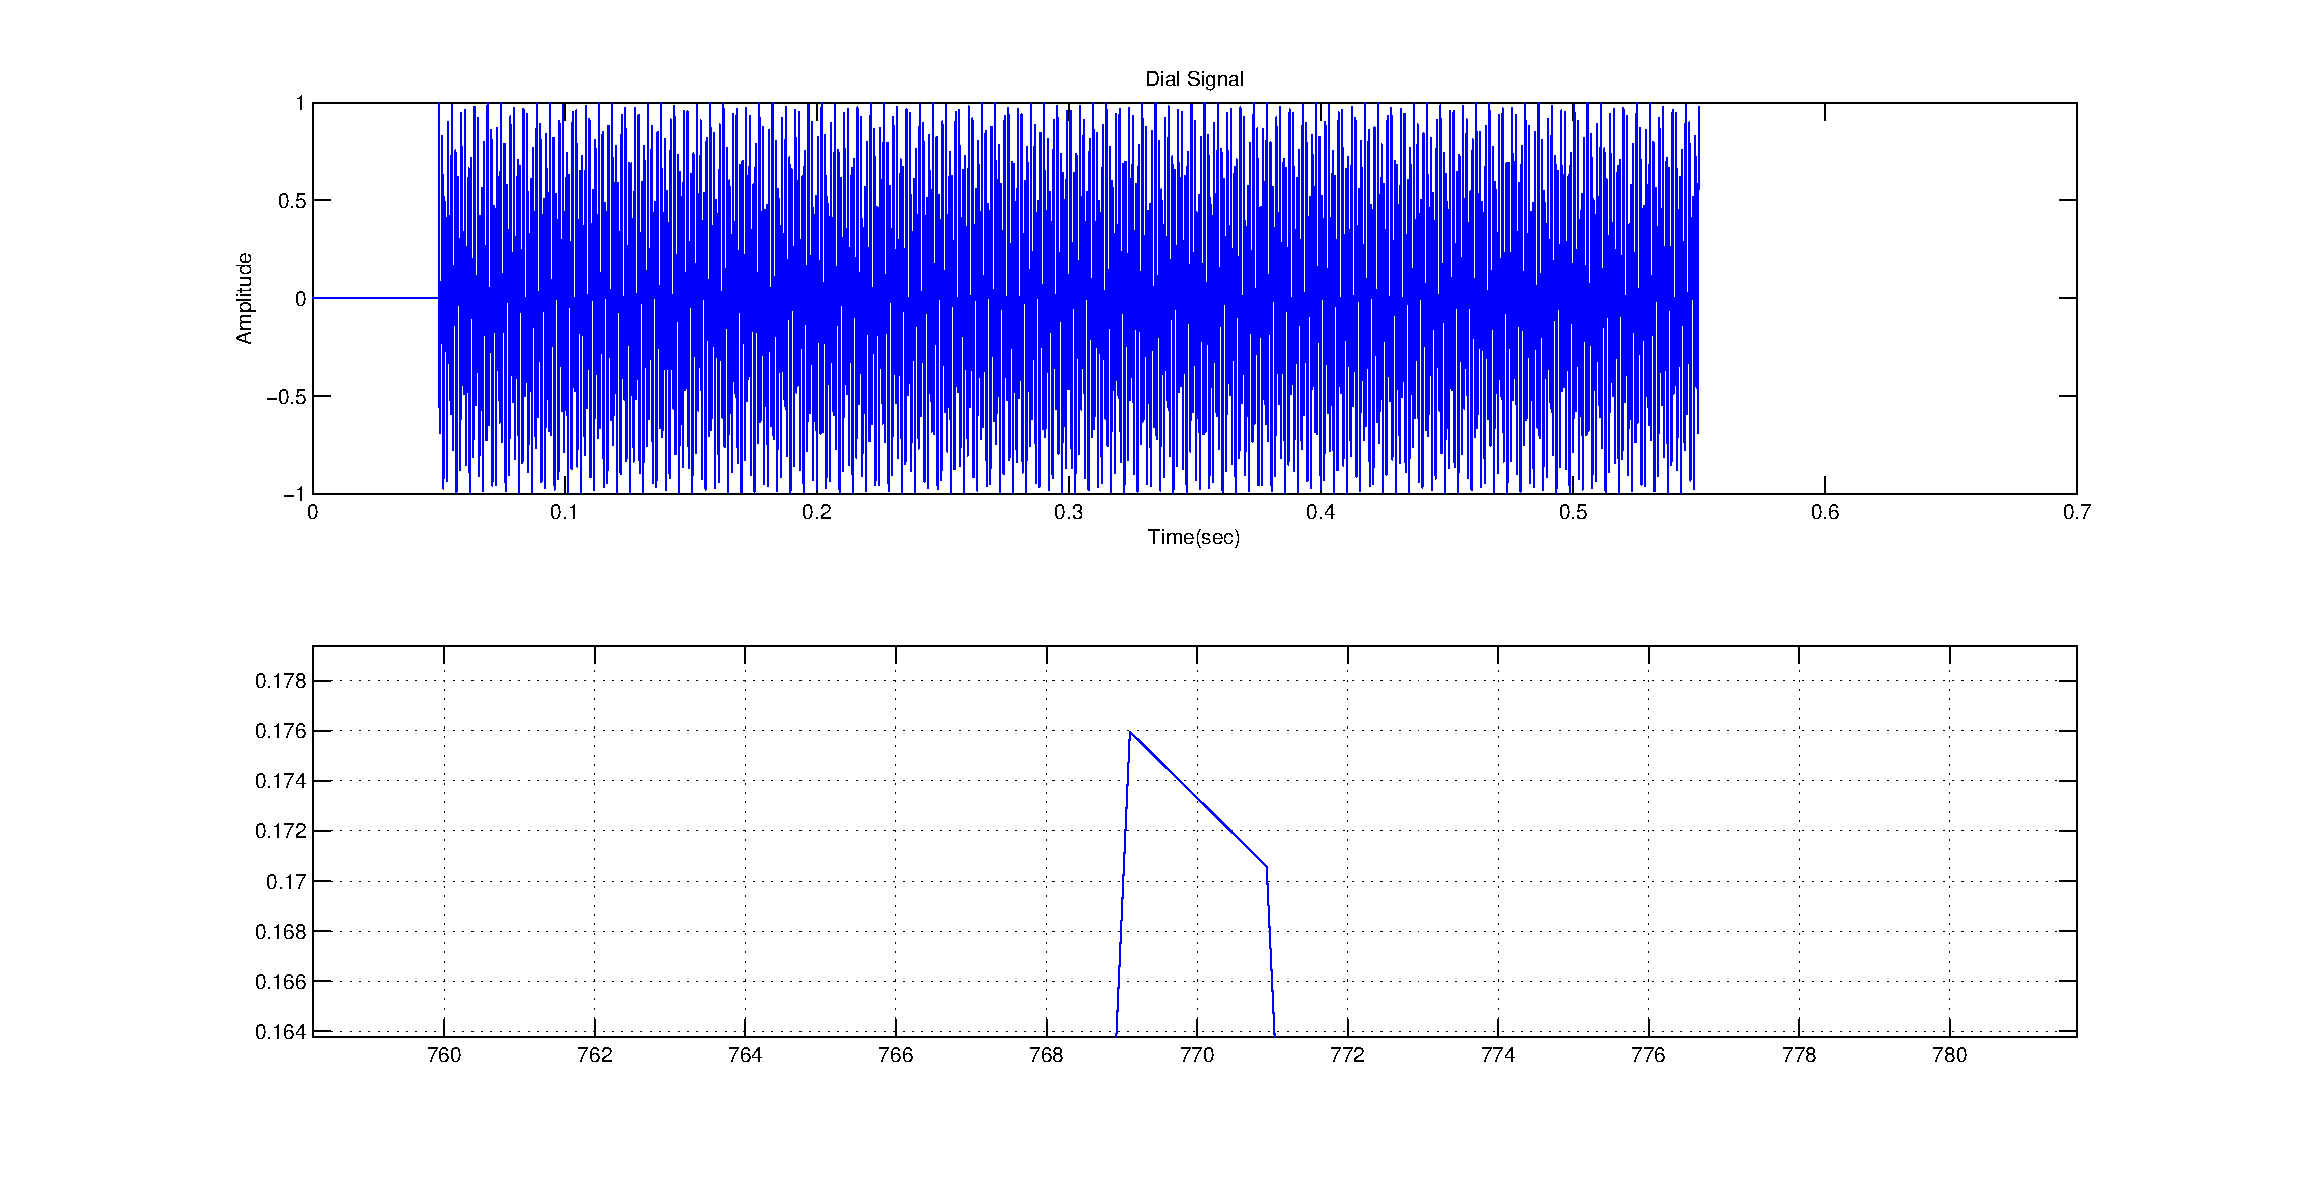
\includegraphics[width=\textwidth]{img43421detail}
                \caption{\texttt{dial\_tones} mit Eingabe \texttt{5}, Zoom bei 770Hz}
            \end{figure}
            \begin{figure}[H]
                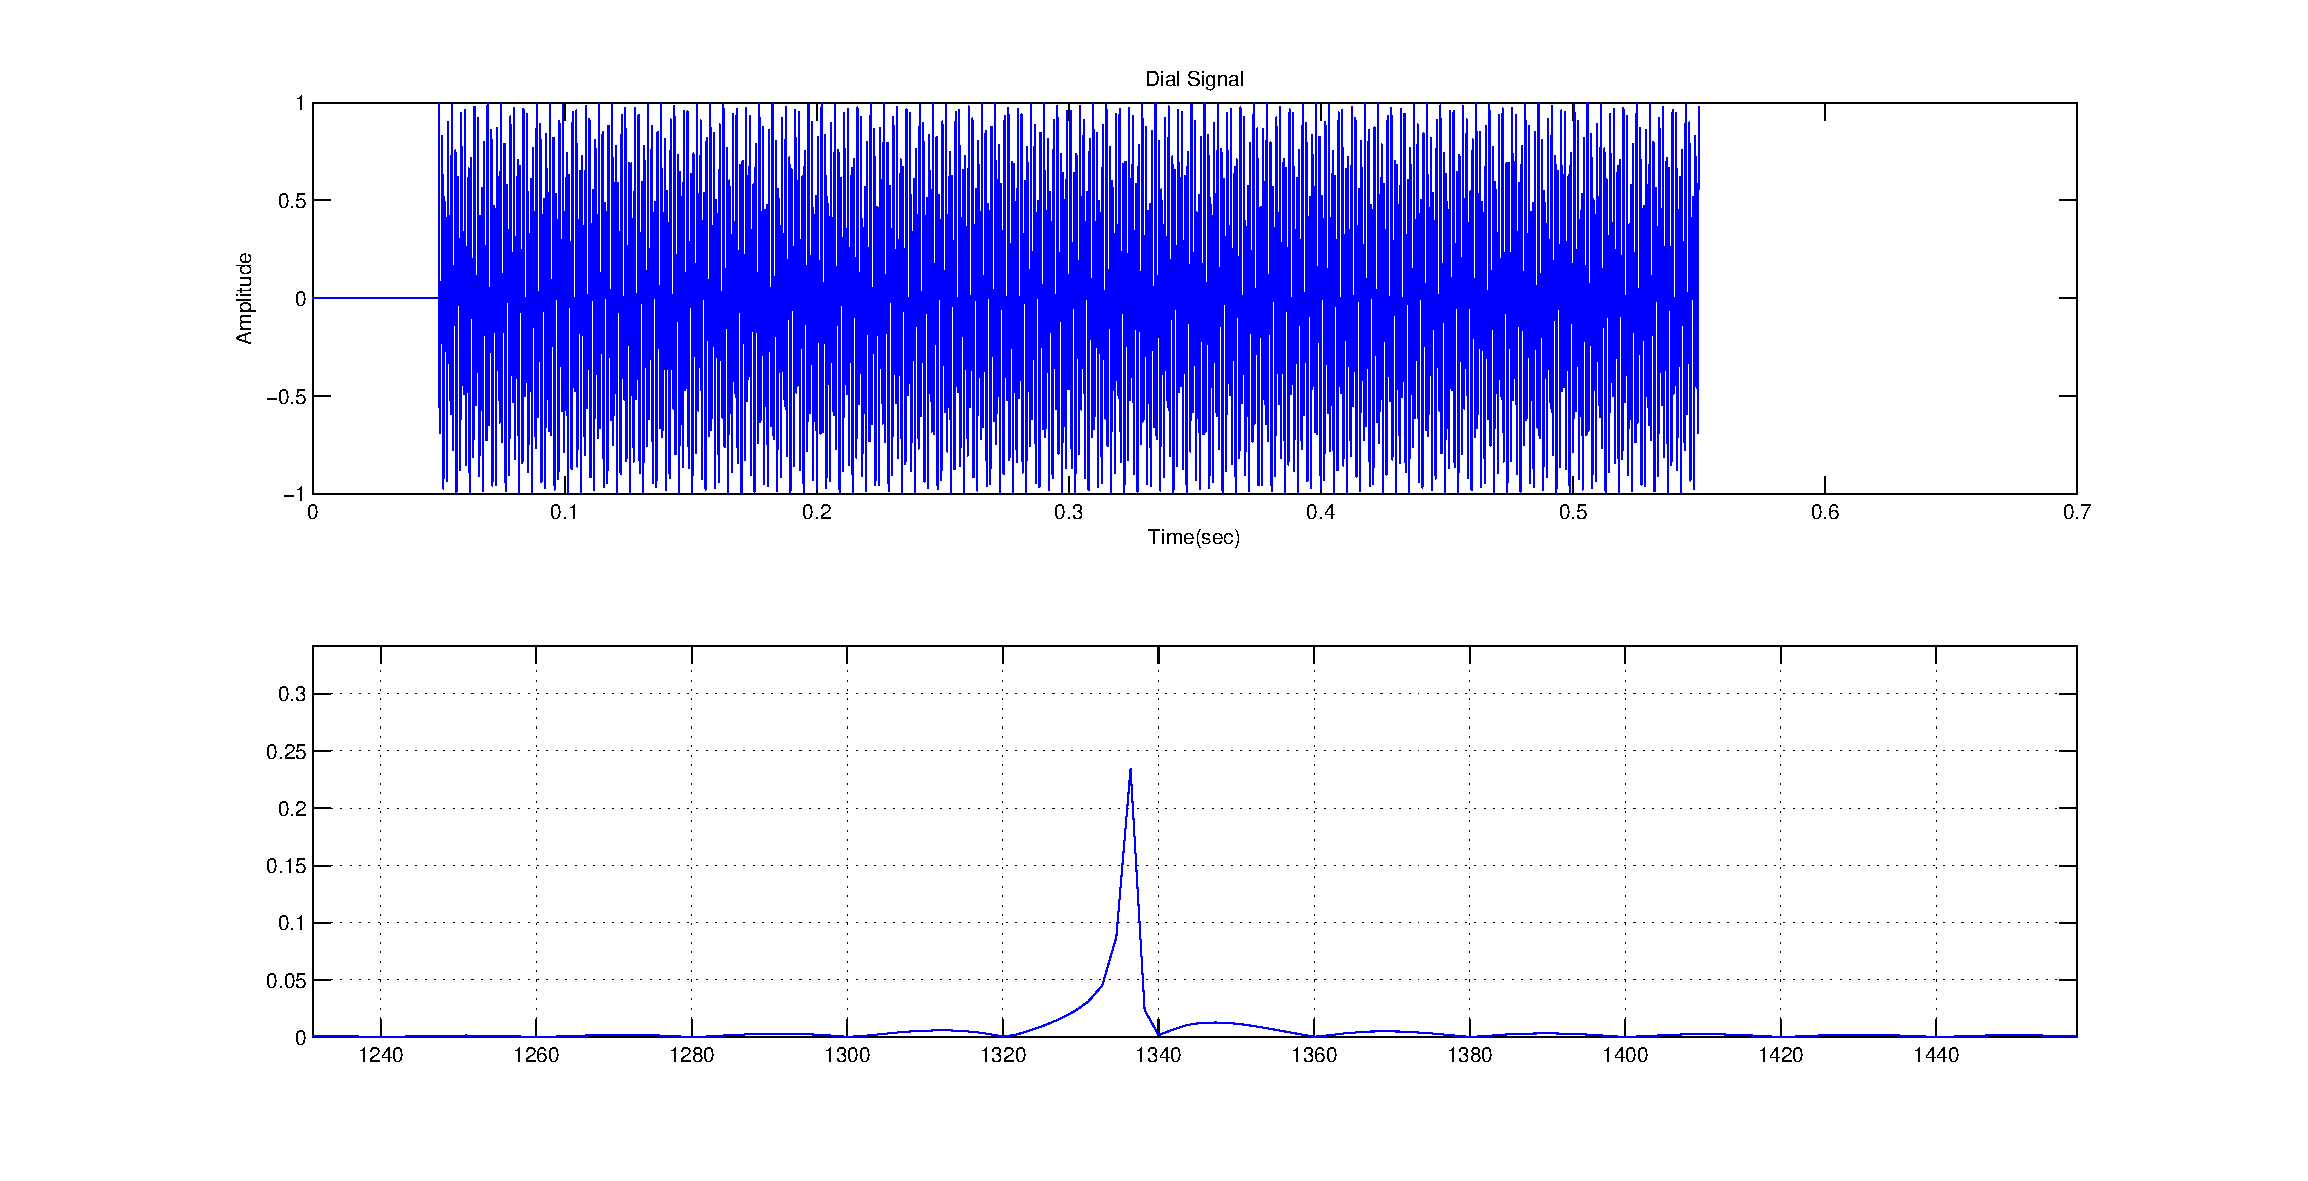
\includegraphics[width=\textwidth]{img43421detail2}
                \caption{\texttt{dial\_tones} mit Eingabe \texttt{5}, Zoom bei 1330Hz}
            \end{figure}
        \end{center}
        Im Frequenzbereich sind die beiden Peaks vergleichsweise breit. Das heißt, die
        Frequenzbestimmung ist ungenauer (eventuell durch Rundungsfehler verursacht).
        Trotzdem ist die gedrückte Taste einwandfrei bestimmbar, da der Peak immer noch
        sehr nah an der gewünschten Frequenz liegt und die verschiedenen Frequenzen
        außreichend große Abstände haben.

        \vspace{2cm}

        \begin{center}
            \begin{figure}[H]
                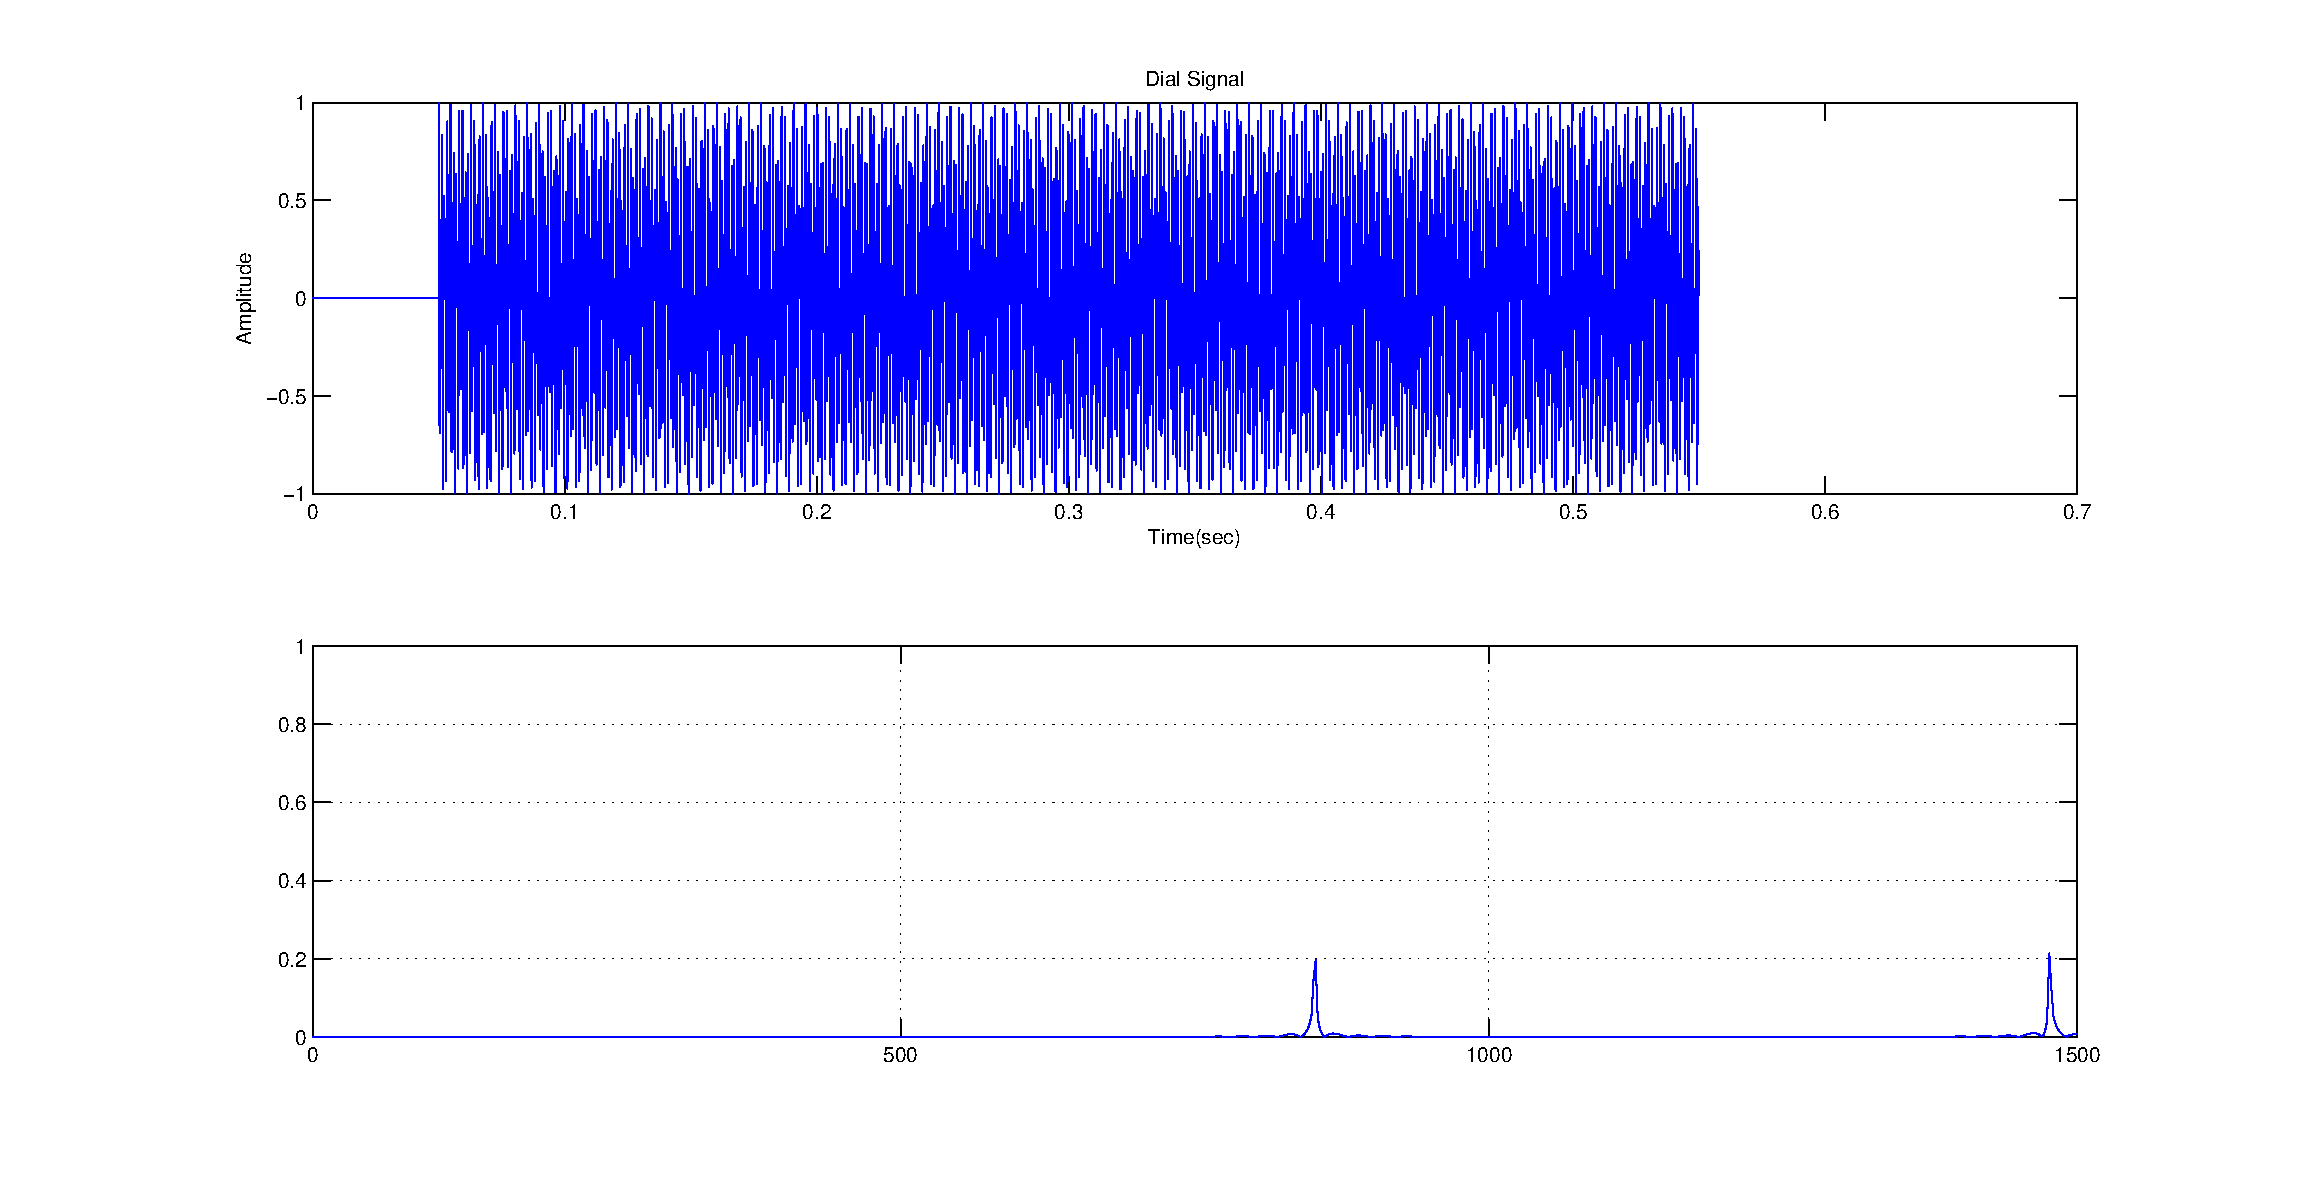
\includegraphics[width=\textwidth]{img43422}
                \caption{\texttt{dial\_tones} mit Eingabe \texttt{9}}
            \end{figure}
        \end{center}

        Da sich die Taste 9 weder in der gleich Zeile, noch in der gleichen Spalte wie
        Taste 5 befindet, sind beide Frequenzen, wie zu erwarten, unterschiedlich.

        \subsection{Identifikation einer unbekannten Nummer}
        \paragraph{Einführung}
        Das in der Datei \texttt{dialed\_number.mat} gespeicherte Signal enthält das DTMF-Signal einer
        12-stelligen Telefonnummer.


        \subsubsection{Import}
        \paragraph{Aufgabe}
        Importieren Sie das Signal in MATLAB und hören Sie es sich mit Hilfe der Funktion
        \texttt{soundsc} an. Zusätzlich zur Variablen \glqq{}number\grqq{} muss für \texttt{soundsc} die Abtastrate
        von 32 768 Hz übergeben werden.

        \subsubsection{Code vervollständigen}
        \paragraph{Aufgabe}
        Die Funktion \texttt{fft\_dtmf.m} enthält einige Fragmente die vervollständigt werden sollen
        um das gesamte DTMF Signal in Zeit- und Frequenzbereich plotten zu können. Vervollständigen Sie den Code. Hinweis: eine solche Funktion ist bereits in
        \texttt{dial\_tones}
        implementiert, es müssen lediglich die entsprechenden Zeilen kopiert werden.
        \paragraph{Protokoll}

        Vervollständigter Code:

        \lstinputlisting[language=Matlab]{fft_dtmf_Student.m}

        \subsubsection{Identifikation der Nummer mittels FFT}
        \paragraph{Aufgabe}
        Ist es möglich mittels der Fourier Transformation über das gesamte Signal die
        gewählte Nummer zu identifizieren? Falls nein, wie muss statt dessen vorgegangen werden?

        \paragraph{Protokoll}
        Da im Frequenzbereich nicht sichtbar ist welche Frequenzen zu welcher Zeit
        im Signal vorhanden war, lassen sich die Nummern nicht aus dem gesamten
        Signal rekonstruieren.

        Das Signal muss nach jedem Ton getrennt werden, damit die einzelnen Segmente
        separat untersucht werden können. Dann sind pro Segment nur zwei Peaks im
        Frequenzbereich sichtbar, aus denen sich dann die gedrückte Taste rekonstruieren
        lässt.

        \subsubsection{Plot}
        \paragraph{Aufgabe}
        Ermitteln Sie nun unter Verwendung von \texttt{receive\_dial} die Fourier Transformierte
        über die einzelnen Zeitabschnitte. Fügen Sie einen Plot von drei der auftretenden
        Ziffern im Frequenzbereich in das Protokoll ein und geben Sie die Frequenzen sowie
        die gewählten Ziffern an.

        \paragraph{Protokoll}
        \begin{center}
            \begin{figure}[H]
                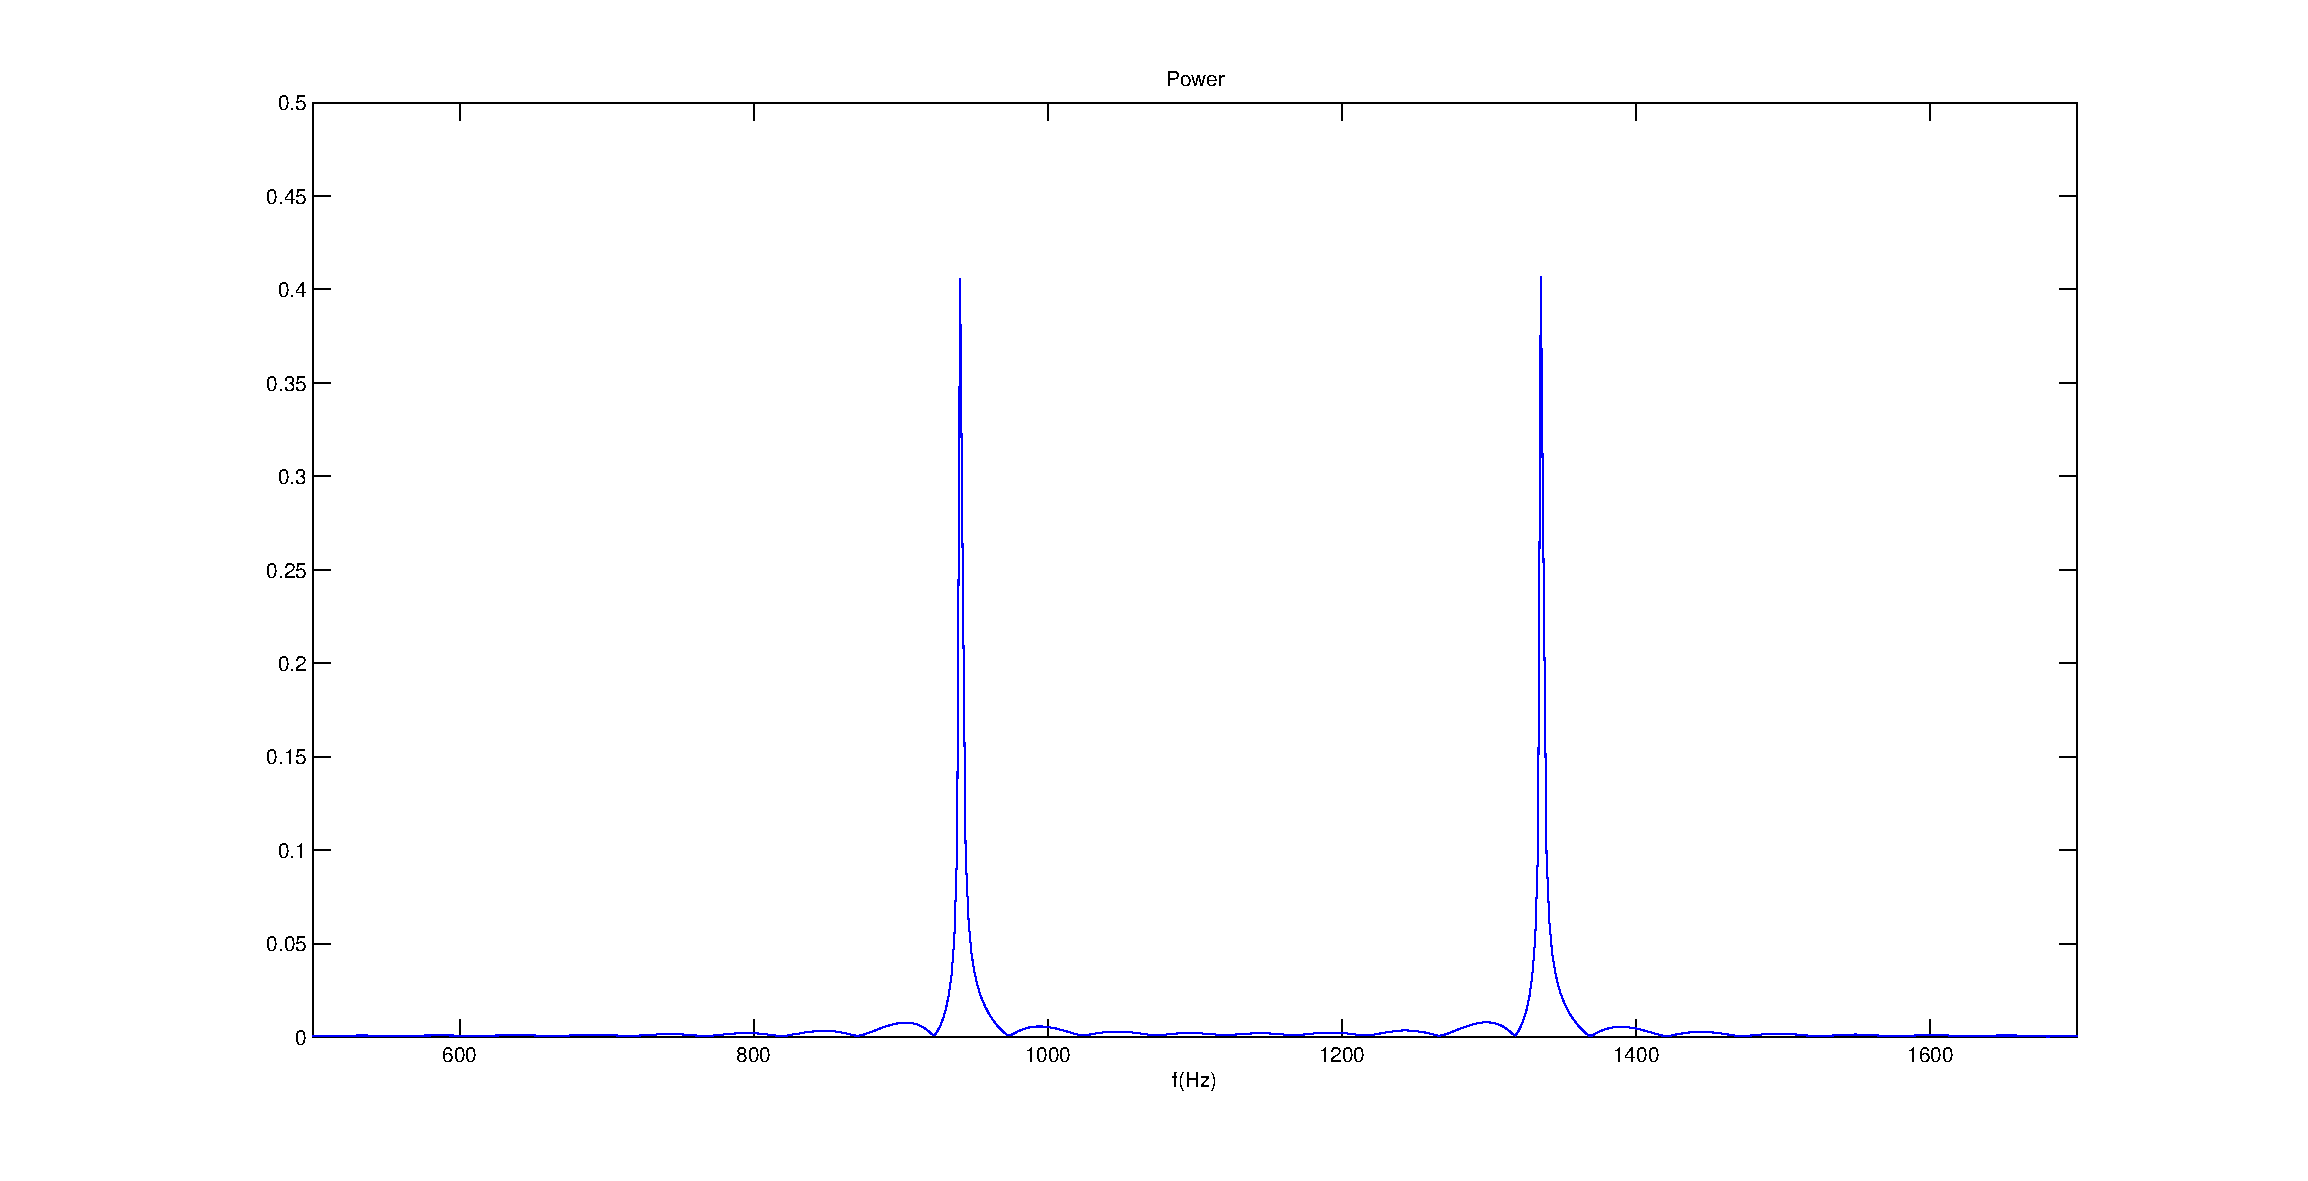
\includegraphics[width=\textwidth]{img43541}
                \caption{Erster Ton mit \texttt{receive\_dial}}
            \end{figure}
        \end{center}
        \begin{eqnarray*}
            f_1 &=& 941 \si{\hertz}\\
            f_2 &=& 1336 \si{\hertz}\\
            &\Rightarrow& \text{Taste: }0
        \end{eqnarray*}

        \begin{center}
            \begin{figure}[H]
                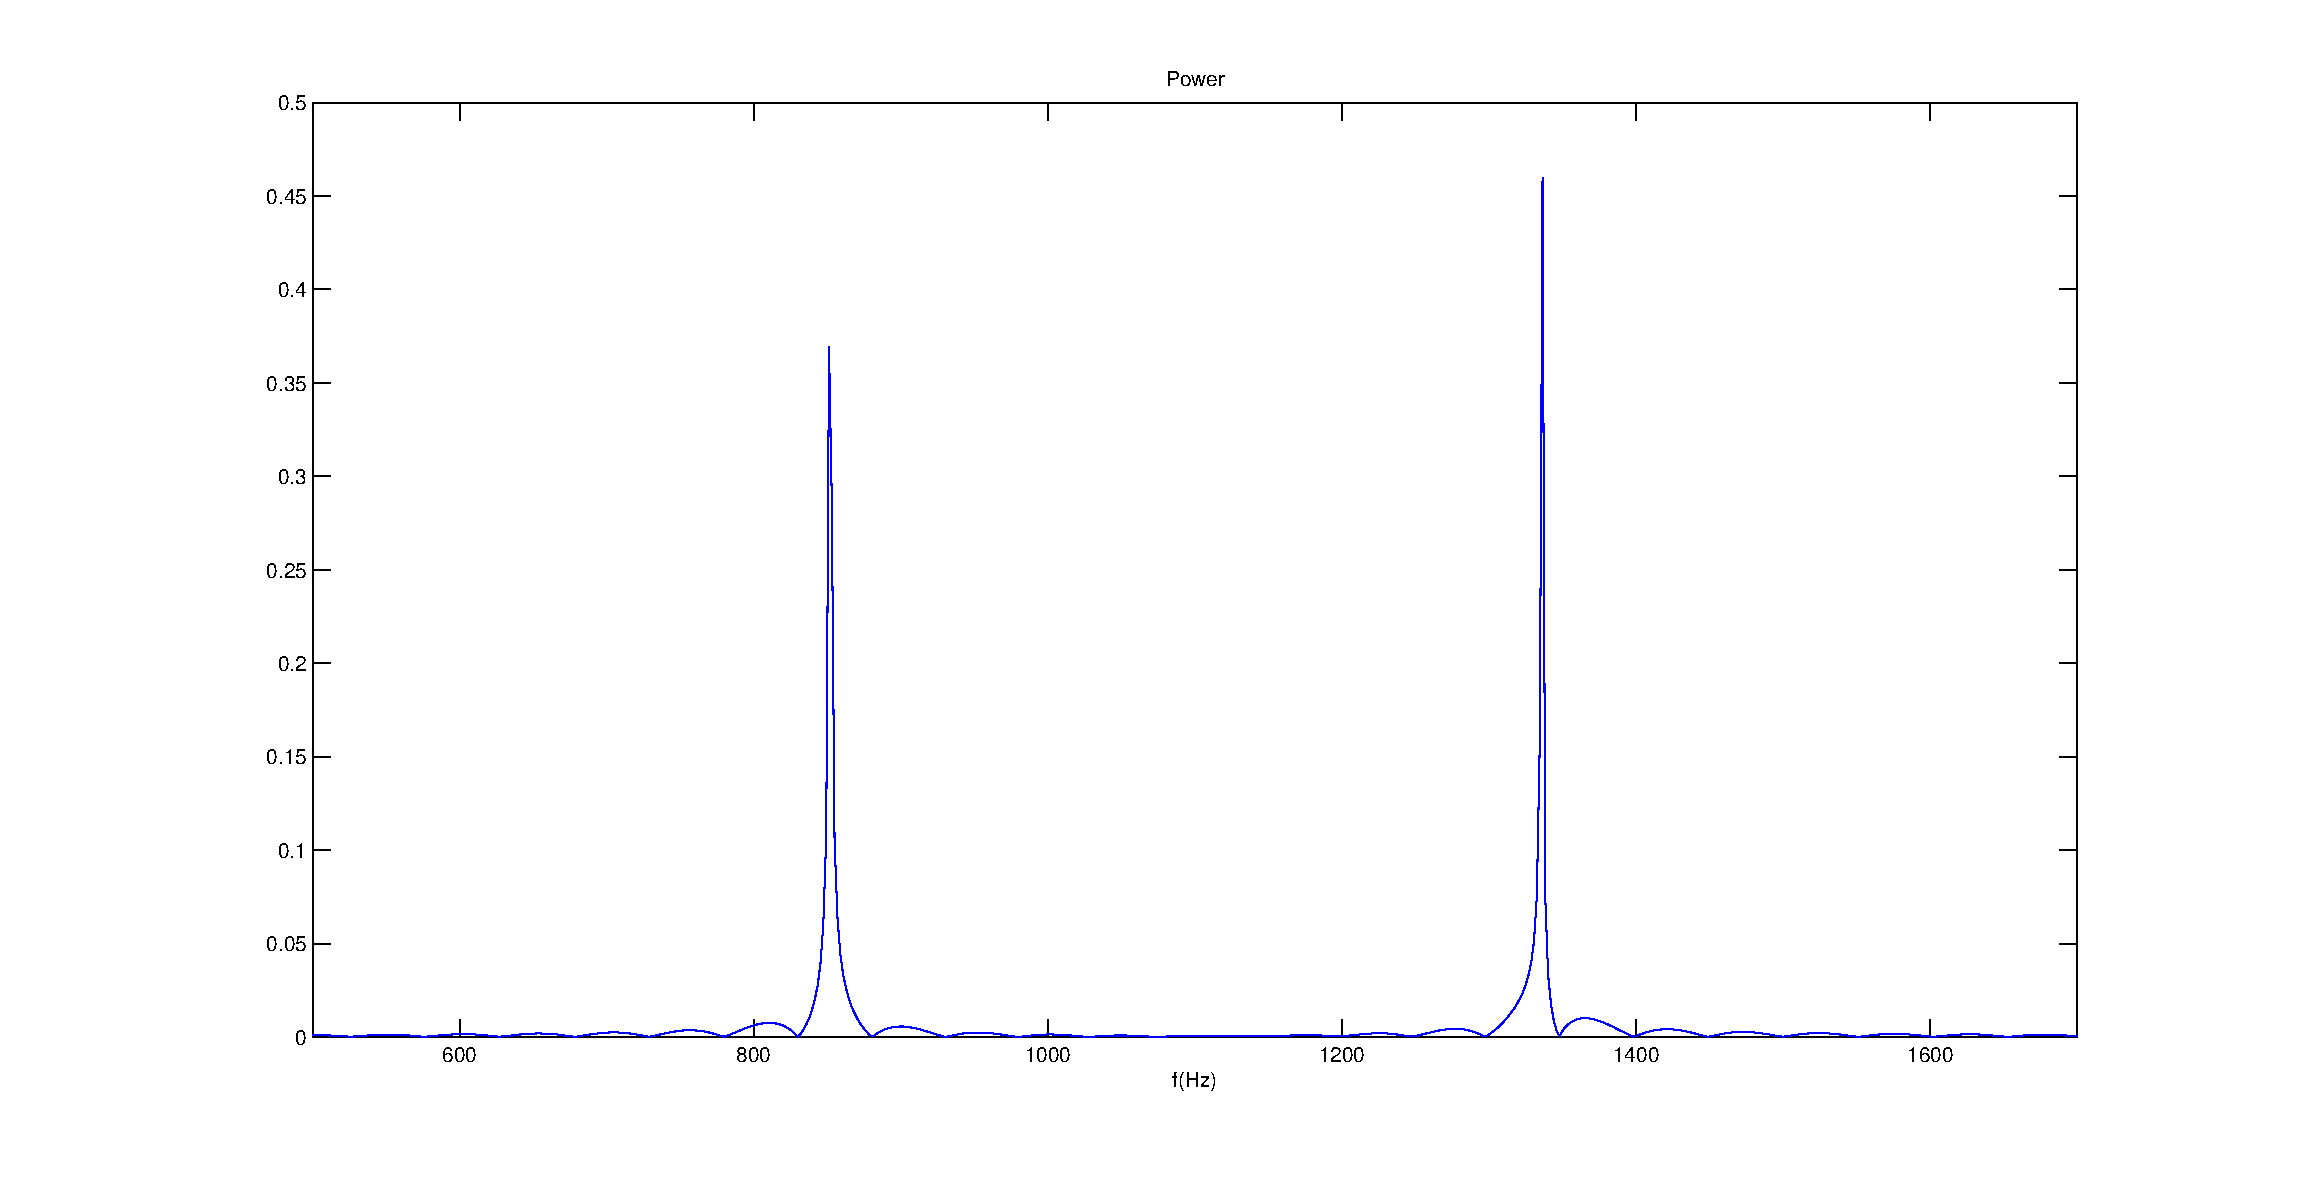
\includegraphics[width=\textwidth]{img43542}
                \caption{Zweiter Ton mit \texttt{receive\_dial}}
            \end{figure}
        \end{center}
        \begin{eqnarray*}
            f_1 &=& 852 \si{\hertz}\\
            f_2 &=& 1336 \si{\hertz}\\
            &\Rightarrow& \text{Taste: }8
        \end{eqnarray*}

        \begin{center}
            \begin{figure}[H]
                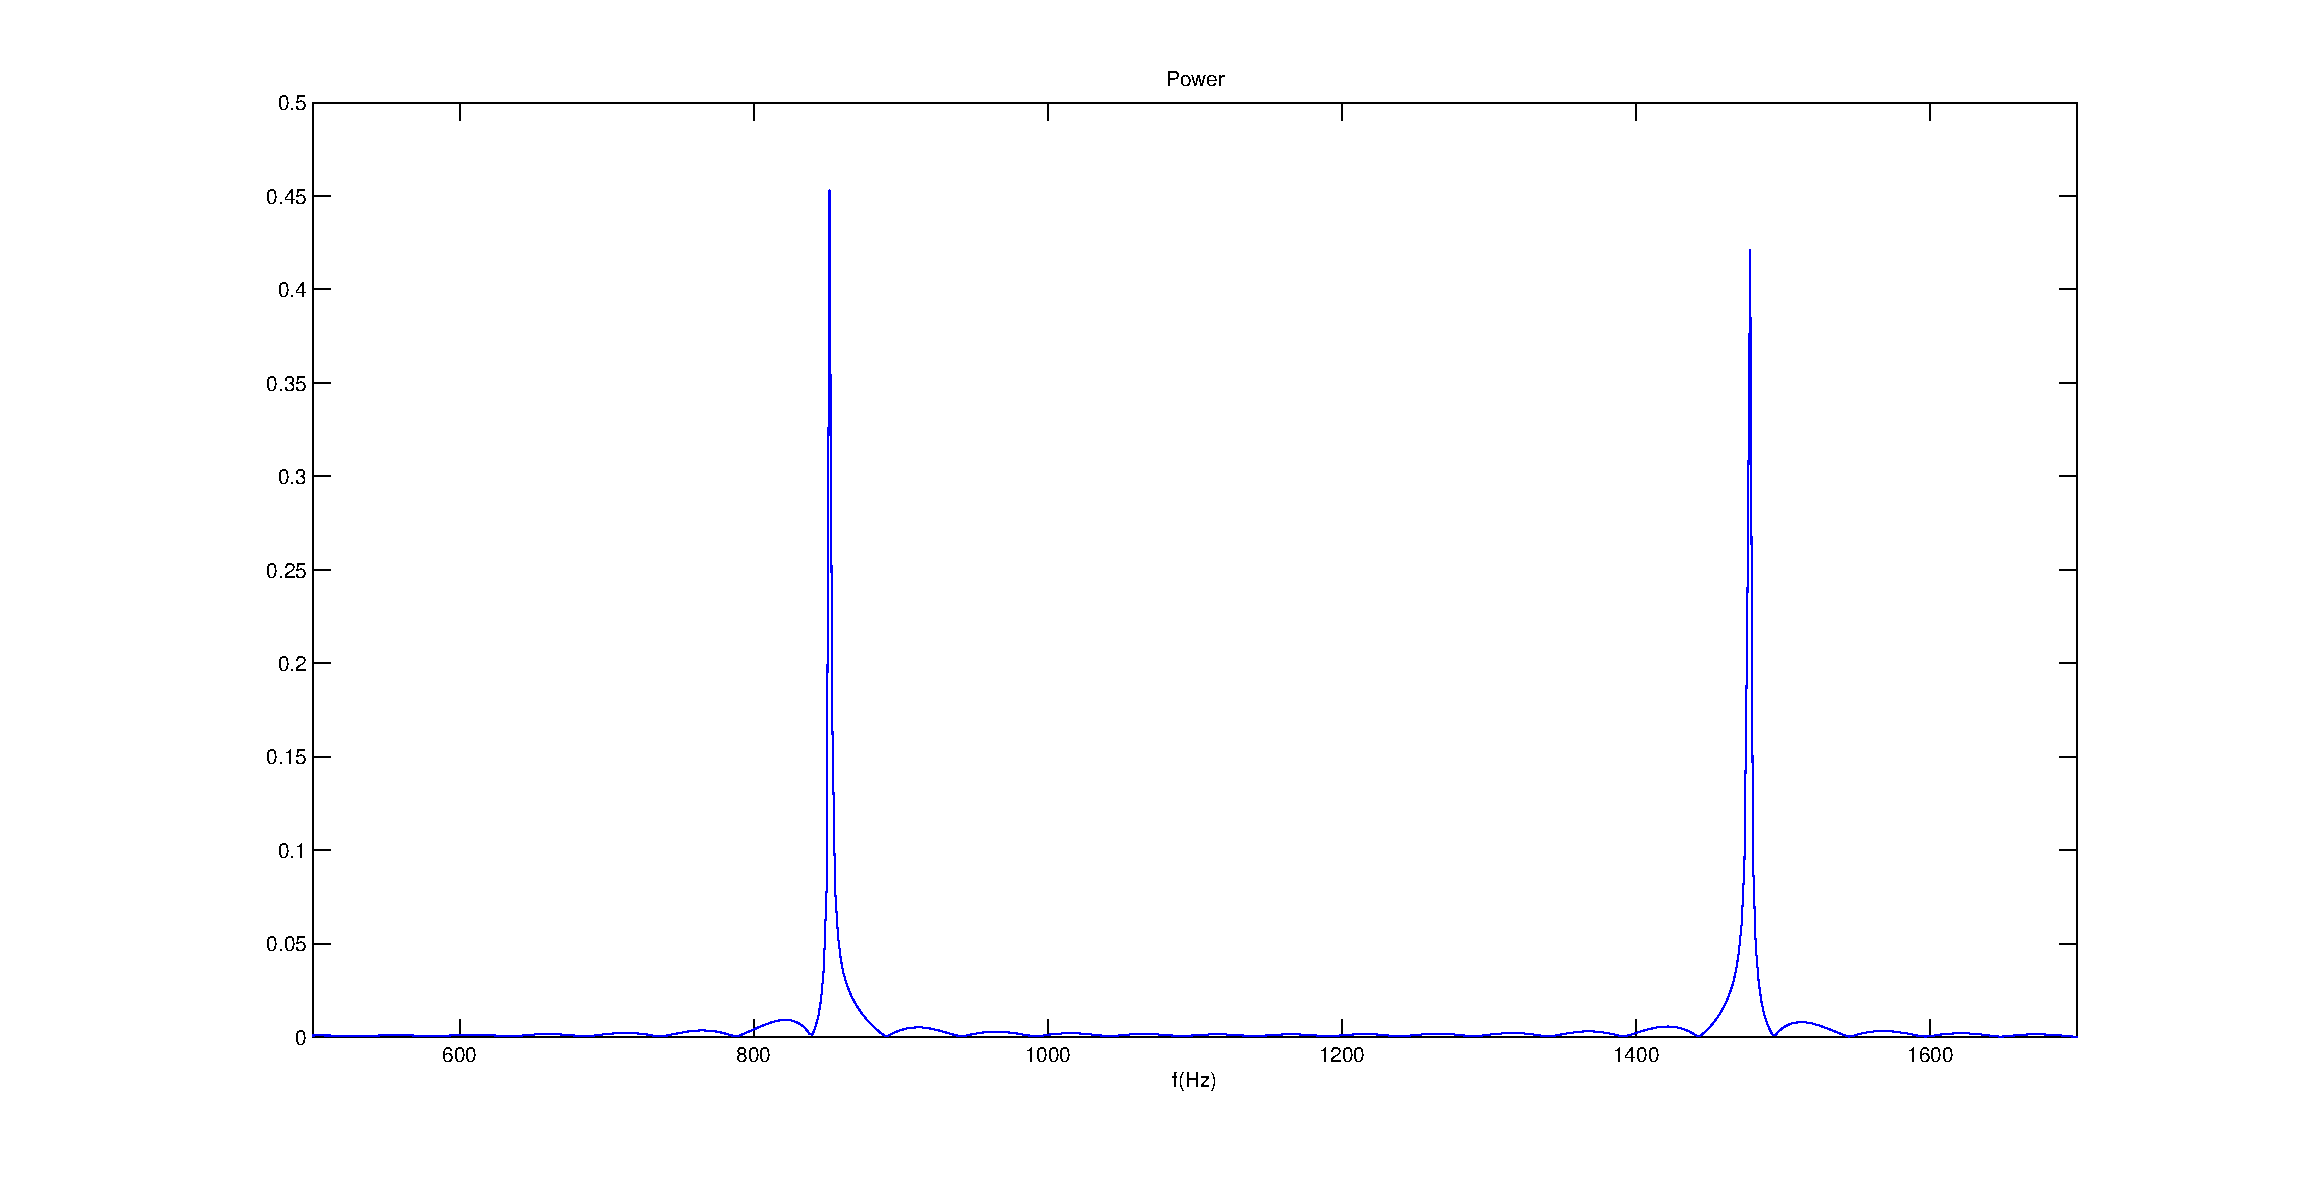
\includegraphics[width=\textwidth]{img43543}
                \caption{Dritter Ton mit \texttt{receive\_dial}}
            \end{figure}
        \end{center}
        \begin{eqnarray*}
            f_1 &=& 852 \si{\hertz}\\
            f_2 &=& 1477 \si{\hertz}\\
            &\Rightarrow& \text{Taste: }9
        \end{eqnarray*}


        \subsubsection{Telefonnummer}
        \paragraph{Aufgabe}
        Wie lautet die gewählte Telefonnummer?

        \paragraph{Protokoll}
        Die Frequenzen wurden jeweils dem Diagramm im Frequenzbereich entnommen
        und daraus die nächst mögliche Tastenfrequenz bestimmt.

        Aus den beiden Frequenzen lässt sich die Taste bestimmen.
        \begin{center}
            \begin{tabular}{ccc}
                \toprule
                $f_1$ & $f_2$ & Taste \\
                \midrule
                941 & 1336 & 0\\
                852 & 1336 & 8\\
                852 & 1477 & 9\\
                770 & 1209 & 4\\
                770 & 1336 & 5\\
                697 & 1336 & 2\\
                697 & 1477 & 3\\
                770 & 1336 & 5\\
                770 & 1477 & 6\\
                852 & 1209 & 7\\
                941 & 1336 & 0\\
                941 & 1336 & 0\\
                \bottomrule
            \end{tabular}
        \end{center}
        Die Nummer lautet:
        \begin{equation*}
            089452356700
        \end{equation*}



        \subsubsection{Code}
        \paragraph{Aufgabe}
        In der Funktion \texttt{receive\_dial} wird das Ergebnis der Fourier Transformierten der
        einzelnen Zeitabschnitte berechnet. In welcher Code Zeile geschieht dies?

        \paragraph{Protokoll}
        Die Fourier-Transformation wird jeweils in Zeile 16 berechnet:
        \lstinputlisting[language=Matlab, firstline=16, lastline=16]{receive_dial.m}


        \subsubsection{Code}
        \paragraph{Aufgabe}
        Wie wird anschließend entschieden um welche Nummer es sich handelt?

        \paragraph{Protokoll}
        Zuerst wird im Frequenzbereich versucht, die Peaks zu identifizieren,
        dann wird für jeden Peak versucht, den Wert einer Taste
        zuzuordnen. Dafür muss die Abweichung von der gemessenen Frequenz zur
        \glqq{}Tastenfrequenz\grqq{} kleiner $2\%$ sein. Aus der Reihen- und
        Spaltenfrequenz kann dann die Taste bestimmt werden.
        \lstinputlisting[language=Matlab, firstline=25, lastline=50]{receive_dial.m}

\end{document}
